\documentclass[12pt]{article}
%\renewcommand{\baselinestretch}{1.15}
\usepackage{natbib,amsmath,amsthm,booktabs,subfigure,anysize,hyperref,graphicx,float,bbm,epstopdf}
\usepackage[margin=1in]{geometry}
\bibliographystyle{aea}
%\bibliographystyle{apalike}
%\bibliographystyle{aernobold}
%\bibliographystyle{economet}
%\marginsize{2cm}{2cm}{2cm}{2cm}

\usepackage{threeparttable}
\usepackage{array} % for adding extra space between table columns
\usepackage{booktabs} % for adding extra space between table columns
\usepackage{multirow}
\usepackage{xcolor}
\usepackage{bm}
\definecolor{dark-red}{rgb}{0.4,0.15,0.15}
\definecolor{dark-blue}{rgb}{0.15,0.15,0.4}
\definecolor{medium-blue}{rgb}{0,0,0.5}
\definecolor{ChadBlue}{rgb}{.1,.1,.5}
% Chad's colors:
% See http://web.njit.edu/~kevin/rgb.txt.html for possibilities
\definecolor{ChadDarkBlue}{rgb}{.1,0,.1}
\definecolor{ChadBlue}{rgb}{.1,.1,.5}
\definecolor{ChadRoyal}{rgb}{.2,.2,.8}
%\definecolor{ChadGreen}{rgb}{0,.35,.1}
%\definecolor{ChadGreen}{rgb}{0,.5,.25}  % Too bright
%\definecolor{ChadGreen}{rgb}{0,.4,.2}    % Still too bright
\definecolor{ChadGreen}{rgb}{0,.4,0}    % Dark Green
%\definecolor{ChadRed}{rgb}{.8,.1,.2}    % Too bright
\definecolor{ChadRed}{rgb}{.5,0,.5}  % purple
\hypersetup{
    colorlinks, linkcolor=ChadRed,
    citecolor=ChadBlue, urlcolor=ChadBlue
}
\newcommand\posscite[1]{\citeauthor{#1}'s (\citeyear{#1})}
\setlength{\parskip}{0.15cm}
\newtheorem{proposition}{\color{ChadGreen} Proposition}
\newtheorem{finding}{\color{ChadGreen} Finding}
\newtheorem{SF}{\color{ChadGreen} Stylized fact}
\newtheorem{hyp}{Hypothesis}
\newtheorem{fact}{Fact}
\newtheorem{prop}{Proposition}
\usepackage{caption}
%\usepackage[font=small,labelfont={color=ChadBlue,bf}]{caption}
\usepackage[font=small,labelfont=bf]{caption}
%\usepackage{subcaption}
%\usepackage{subfloat}
\usepackage{amssymb}
\usepackage{amsfonts}
\usepackage{amsmath}
\usepackage{accents}
\usepackage{color,soul}
\usepackage{smartdiagram}
\usepackage[figuresright]{rotating} % Rotating table
\usepackage{lscape} % Rotating table
\usepackage{diagbox}
\usepackage{multicol}
\usepackage{tikz}
\usepackage{comment}
\usepackage{float}

\newcommand{\ubar}[1]{\underaccent{\bar}{#1}}
\usepackage{setspace}  %using this package conflits with footnote hyperlink jump. Using this package makes the footnote links inactive.
\usepackage[all]{hypcap}        % needed to help hyperlinks direct correctly;
%\renewcommand{\sfdefault}{ptm}

\newtheorem{theorem}{Theorem}
\newtheorem{cor}[theorem]{Corollary}
\renewcommand{\proof}{\noindent \textbf{Proof.\ }}
\newtheorem{conjecture}{Conjecture}
\newtheorem{example}{Example}
\newtheorem{defn}{Definition}
\renewcommand{\qed}{\hfill\rule{2.1mm}{2.1mm}}
%\newtheorem{proposition}{\color{ChadGreen} Proposition}
%\newtheorem{finding}{\color{ChadGreen} Finding}
%\newtheorem{SF}{\color{ChadGreen} Stylized fact}
% Fix title, sections, etc.
\newcommand\fnote[1]{\captionsetup{font=small}\caption*{#1}}

\let\LaTeXtitle\title
%\renewcommand{\title}[1]{\LaTeXtitle{\color{ChadBlue}{\LARGE #1}}}
%\renewcommand{\abstractname}{\color{ChadBlue}Abstract}
%\renewcommand{\figurename}{\color{ChadBlue}Figure}
%\renewcommand{\tablename}{\color{ChadBlue}Table}
\renewcommand{\arraystretch}{1.1} % space between rows

\usepackage{sectsty}
%\allsectionsfont{\color{blue}\itshape\underline}
%\sectionfont{\color{ChadBlue}}
%\subsectionfont{\color{ChadBlue}}
%\subsubsectionfont{\color{ChadBlue}}
\usepackage{lscape}
\graphicspath{{figure/}}
\newcolumntype{P}[1]{>{\centering\arraybackslash}p{#1}}

%\newcommand\YUGE{\fontsize{30}{40}\selectfont}

\linespread{1.2}
\geometry{a4paper,scale=0.75}
\setlength{\parskip}{0.5em}

% comments: 
% add JEL; add Highlights (check JDE requirement)
% Move literature review into introduction and make it shorter 
% 

%---------------------------------------------------------------------------------------

\begin{document}

\title{  \Large \textbf{Exchange Rate Pass-Through and Importers' Credit Constraints: Evidence from China}}

\author{\large \href{http://yaoli.people.ust.hk/}{Yao Amber Li}\thanks{Li: Department of Economics and Faculty Associate of the Institute for Emerging Market Studies (IEMS), Hong Kong University of Science and Technology, Clear Water Bay, Kowloon, Hong Kong SAR-PRC. Email: \href{mailto:yaoli@ust.hk}{yaoli@ust.hk}.}\\ \large{HKUST}
\and \large \href{}{Lingfei Lu}\thanks{Lu: Department of Economics, Hong Kong University of Science and Technology, Clear Water Bay, Kowloon, Hong Kong SAR-PRC. Email: \href{mailto:}{lingfei.lu@connect.ust.hk}.} \\ \large{HKUST}
 }

\date{\today }

\maketitle

\begin{abstract}
Exchange rate fluctuations are a key factor affecting international trade prices. This paper studies the incomplete exchange rate pass-through patterns in China and its linkage with importers' credit constraints. Using Chinese firm-level information and customs transaction records from 2000 to 2007, we find that (1) the average import price pass-through in China is about 65\% to 73\%, far below the near complete (94\%) export price pass-through; (2) for importers in financially more vulnerable industries, exchange rate pass-through tend to be more complete; (3) a higher degree of import source diversity can effectively lead to a less complete pass-through and offset the effects of credit constraints. This suggests that a more diverse sourcing network can alleviate the impact of financial market imperfections on trade.\\
(\textit{JEL} F14, F31, F41)

\end{abstract}

\section{Introduction} \label{Introduction}

Why do exchange rate fluctuations not result in price changes of the same magnitude? This is one of the core questions among a set of ``exchange rate disconnect'' puzzles (\cite{obstfeld2000}). As price signals in the international trade market, exchange rates appear less informative for firms than expected. Exchange rate pass-through (ERPT), which describes the elasticity of local price changes to exchange rate fluctuations, varies widely across countries, industries, and time. Existing studies have generated widely varying estimates of the exchange rate pass-through. It is of particular interest to researchers both in the fields of international trade and open macroeconomics to demystify the ``exchange rate disconnect" puzzles. Understanding the pattern of exchange rate pass-through has important implications for formulating macro policy, including monetary policy, inflation targeting, and the balance of payments.

In this paper, we focus on the role of importers in the determination of exchange rate pass-through and connect it with the importers' financial constraints. This paper tends to fill a gap in the literature by linking both sides of the trade relationship and provides a novel perspective to study the nature of exchange rate disconnect for emerging markets, where firms are more vulnerable to credit constraints due to immature financial markets. In contrast to the conventional framework of exchange rate pass-through where importers are mostly price takers, we contribute to the literature by identifying the importers' implicit sourcing power and comparing their heterogeneous capacity to absorb exchange rate shocks. Throughout the paper, we will compare firm-level import exchange rate pass-through with export pass-through to reflect the similarities and differences between the two. Going a step further, if a country's export and import exchange rate pass-through patterns differ significantly, this may even affect terms of trade as well as current account imbalances. We believe that micro-evidence from import exchange rate pass-through provides a new perspective to study the ``exchange rate disconnect" puzzle.

We estimate the exchange rate pass-through as the price elasticity of import prices concerning real exchange rates using Chinese micro-level data. Specifically, we merge the Chinese Industrial Enterprises datasets with the transaction data from China’s customs and adopted fixed effects panel regressions with first-order differences to capture the changes in product prices and real exchange rates. The average import exchange rate pass-through is between 35\%-40\%, which is obviously less complete compared to the over 95\% export pass-through. Second, we identify the effects of credit constraints on importers' exchange rate pass-through. We use US measures of sectors’ financial vulnerability (\cite{manova-wei-zhang2015}) in our main empirical analysis while use Chinese measures of credit needs (\cite{fan-li-yeaple2015}) for robustness checks. In our baseline results, import prices for firms in sectors with higher financial constraints are more sensitive to exchange rate shocks. Third, we calculate the proxy for an importer's sourcing base and find that an importer with more alternative importing options can resist the effects of credit constraints and absorb exchange rate shocks better.

In the discussion part, we control several potential factors which may affect the import pass-through other than credit constraints. We first estimate the firm-level markup estimated following \cite{dlw2012} and test how markups affect import ERPT. In addition, firms with different market shares also demonstrate heterogeneous price responses to exchange rate changes. We confirm that although firm heterogeneity in those aspects does affect exchange rate pass-through, credit constraints still play a role that cannot be ignored even after we control those firm characteristics. In robustness checks, we further use alternative measures of credit constraints and alternative subsamples. For alternative measures, we compare sector-level credit constraints variables calculated from China data with those from US data. For alternative samples, we divide our subjects into two subsets: two-way traders (simultaneous import and export) and one-way traders (either only import or only export). We check our results using only the two-way traders who account for the vast majority of trading firms and the vast majority of China's trade volume. These results are all significant and robust.

We show that importers‘ credit constraints do influence price-setting patterns in international trade. We provide evidence for three key findings: (1) the average import exchange rate pass-through level in China is significantly less complete than the export one; (2) financial constraints will increase both of them to be more complete, and (3) importers who import a certain product from more sources have a less complete pass-through. In other words, financially constrained importers will absorb more price fluctuations caused by exchange rate changes, while financially constrained exporters pass through more exchange rate changes to prices, both compared to those unconstrained firms. This reflects that binding financial constraints will lead to not only narrow margins to adopt pricing-to-market strategies for the sellers but also limited sourcing power for the buyers. Importers with a wider sourcing base could get more access to alternative options and avoid bargaining disadvantages in exchange rate fluctuations to some extent.

This paper contributes to three strands of literature. First, this paper contributes to a wide literature on exchange rate disconnect (\cite{obstfeld2000}), particularly on trade pricing response to exchange rate changes (\cite{campa2005}). Trade prices denominated in the destination currency are usually much less volatile than exchange rates. Recently, more studies link the exchange rate pass-through to disaggregated firm-level characteristics. \cite{bmm2012} find that exporters with better performance react to an exchange rate shock by adjusting more their markup and less their export volume. \cite{aik2014} find that firms with higher import intensity and larger market share have less complete price pass-through. Many follow-up works find that exporters' productivity (\cite{lmx2015}) and product quality (\cite{chen2016}; \cite{auer2018}), as well as their imported inputs (\cite{wang-yu2021}), market shares (\cite{auer2016}; \cite{devereux2017}) and information access (\cite{garetto2016}), will all affect the export exchange rate pass-through. For Chinese exporters, \cite{lmx2015} find nearly complete exchange rate pass-through into RMB price for Chinese exporters, which means that their domestic currency price response is very weak. Yet the role of importers in determining exchange rate pass-through remains a novel field to study. The contribution of this paper is to provide micro-level evidence of importers' heterogeneity in response to exchange rate shocks when firms are operating in industries with varying degrees of credit constraints. This supports the idea that international trade pricing is influenced by the characteristics of both importers and exporters. We believe that the bargaining power of importers, an important yet underexplored force that determines pricing patterns in the international market, may help explain the exchange rate disconnect puzzle. 

Second, we contribute to the literature by analyzing how credit constraints affect the exchange rate elasticity to international prices. We study the influence of sector-level credit constraints on the response of import prices to exchange rate fluctuations. The most relevant study to this paper is \cite{strasser2013}, which discusses the relationship between exchange rate pass-through and exporters' credit conditions. \cite{strasser2013} uses a firm-level survey to show that financially constrained exporters pass exchange rate shocks to prices more completely. Subject to variable markups, firms under borrowing constraints must keep the pricing-to-market (PTM) strategy to a limited extent because they have less space to adjust their profit margin. One recent article \cite{dai2021} finds that exchange rate pass-through to export prices denominated in home currency is lower for firms under tighter financial constraints. However, they focus on firm-level aggregate export behaviors while we assess the bilateral trade elasticity with each country instead. Our paper differs from earlier studies in that, first, we focus on importers, whose pricing behaviors are also affected by credit constraints, and second, with the detailed Chinese panel data, we could estimate the relationship between credit constraints and price response to exchange rate shocks at firm-source-product-year level controlling for various associated variables and their interactions. In addition, we provide a novel perspective to study the exchange rate disconnect puzzle in emerging markets, where firms are usually financially more vulnerable due to immature financial markets.

Third, this paper relates to the broader literature on credit constraints and international trade. The cross-border transportation of exporting or importing is riskier than domestic sales or purchasing, and contractual reliability in international transactions is weaker. Therefore, it is widely believed that trade participants rely on additional external capital to pay fixed costs to source from or export to other countries, which can not be fully covered by internal cash flows from operations (\cite{manova2013}, \cite{chaney2016}). \cite{feenstra-li-yu2014}, \cite{manova-wei-zhang2015}, \cite{fan-lai-li2015}) provide comprehensive theoretical explanations and empirical evidence from China about how credit constraints affect exports, through incomplete information, multinational links, and quality, respectively. Recently, \cite{xu-guo2021} demonstrate that the estimated exchange rate elasticity of export volume is negatively correlated with the sector’s degree of financial constraints. However, controlling markup adjustment could not fully eliminate the effect of financial constraints, which leaves room for further research. In the context of exchange rate shocks, our study deliberately examines how credit constraints affect the robustness of importers' global sourcing behavior. This provides a novel perspective to study the exchange rate disconnect puzzle in emerging markets, where firms are usually financially more vulnerable due to immature financial markets.

The remainder of this paper is organized as follows. Section \ref{Data&Measurements} describes the data and measurements of key variables. Section \ref{Empirical} introduces our empirical identification strategies and main results. Section \ref{Robustness} examines the robustness of our results.  Section \ref{Discussion} discusses other factors affecting exchange rate pass-through and their interactions between credit constraints. Section \ref{Conclusion} concludes.

\section{Data and Measurements} \label{Data&Measurements}

This section describes our data and measurements of some key variables. We will also present some summary statistics based on the China's trade data and industry-level credit constraints measures.

\subsection{Data} \label{Data}

We conduct our empirical research using various data sources: (1) country-level macro data from the Penn World Table 10.0 and the International Financial Statistics (IFS), (2) detailed transaction-level data provided by China’s General Administration of Customs, (3) the annual surveys from Chinese Industrial Enterprises provided by the National Bureau of Statistics of China.  In this section, we will introduce the basic information about these datasets.

\subsubsection{Country-level macro data} \label{Data-Macro}

We obtain annual bilateral nominal exchange rates from the newest version of Penn World Table (PWT 10.0) referring to \cite{feenstra2015}, and consumer price indices (CPI) from the International Financial Statistics. We keep all China's trade partners who keep full records of exchange rates and CPI from 1999 to 2011, resulting in 154 countries. Those major countries account for more than 95 \% of Chinese imports and exports.

Following the convention, the bilateral nominal exchange rate ($NER_{ct}$) is defined as the number of home currency units that can purchase a unit of foreign currency. By this definition, an increase in $NER_{ct}$ means a nominal depreciation of the Chinese RMB against this currency from country $c$. Following \cite{lmx2015}, the CPI-based real exchange rate ($RER_{ct}$) is defined as the nominal exchange rate multiplied by the foreign consumer price index and divided by the Chinese consumer price index at the same year, which is

$$
RER_{ct}=NER_{ct} \cdot \frac{CPI_{ct}}{CPI_{CHN,t}}.
$$

Similarly, an increase in $RER_{ct}$ means a real depreciation of the Chinese RMB against the foreign country's c currency. In later specifications, we mainly use the first difference of the logarithm of the real exchange rate to represent exchange rate changes.

Changes in nominal and real exchange rates for the U.S. dollar and the euro relative to Chinese RMB (level in 1999 as base value 100) are shown in figures \ref{fig.USD} and \ref{fig.EUR}. We could observe that the real exchange rates against the US dollar were relatively stable in 2000-2004 due to the nominal pegging scheme of RMB to US dollars. In July 2005, the peg was lifted to a slight appreciation of RMB against US dollars as a result of this exchange policy evolution. However, exchange rates of RMB against Eurozone fluctuated up and down during this period. 

\begin{figure}[htbp]
	\centering
	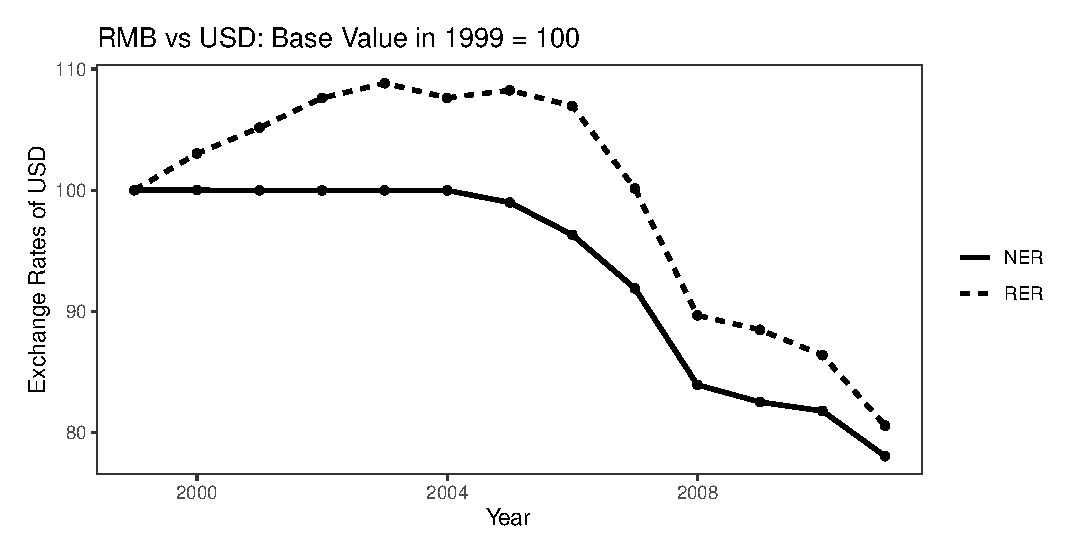
\includegraphics[width=1\textwidth]{R/USD.eps}
	\caption{Exchange rates of Chinese RMB against the U.S. dollar (1999-2011)}
	\label{fig.USD}
\end{figure}

\begin{figure}[htbp]
	\centering
	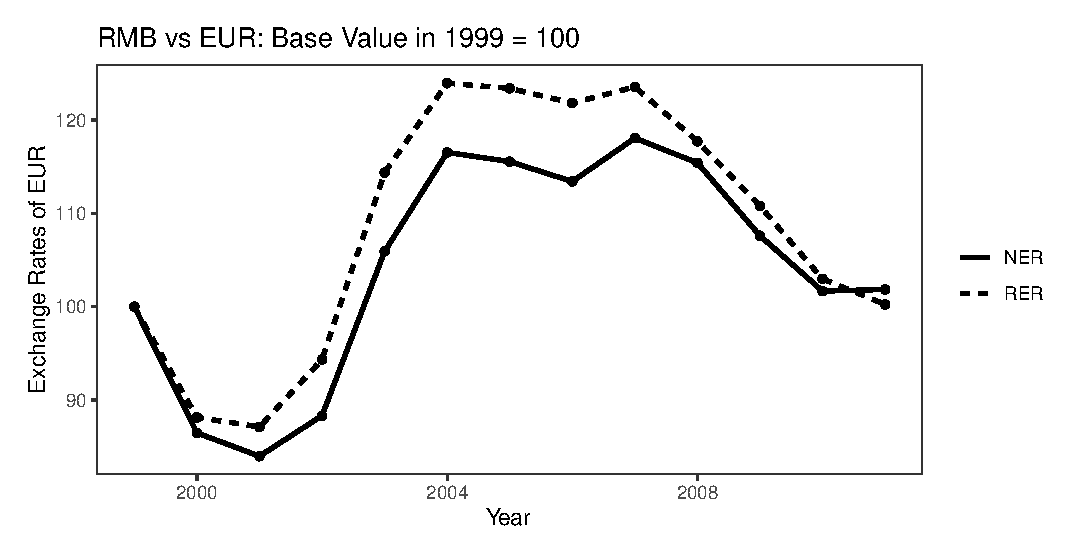
\includegraphics[width=1\textwidth]{R/EUR.eps}
	\caption{Exchange rates of Chinese RMB against euro (1999-2011)}
	\label{fig.EUR}
\end{figure}

In addition to nominal and real exchange rates, we also use the real GDP of foreign countries from PWT 10.0. The real GDP is computed with national-accounts growth rates. The controls of real GDP changes of the destination country, $\Delta RGDP_{ct}$, help us exclude the effect of differential economic growth on price movements. All macro variables including exchange rates and real GDPs are in annual terms to match the firm information.

\subsubsection{Customs transaction-level data} \label{Data-Customs}

The first dataset we use is the transaction-level records from the General Administration of Customs of China (GACC) as in \cite{manova-zhang2012}. The whole sample period ranges from 2000 to 2011. This dataset includes the most comprehensive information on all Chinese trade transactions including each firm's import or export value (denominated in US dollars), quantity, unit, product name and code, source or destination country, and the type of enterprises (e.g., state-owned, private, foreign-invested, and joint ventures), etc. Using these detailed trade records, we are able to compute firm–product unit values to study export or import price responses to exchange rate shocks. 

We separate the full records into export and import parts. In our analysis, each unique transaction refers to a firm-product-country-year consolidation. The categories of products in China's customs trade records are coded according to the Harmonized Coding and Description System (HS) from World Customs Organization (WCO). The original data is subject to HS 8-digit classification. Since there are two major revisions of the HS system in 2002 and 2007, we aggregate HS8 product-level information to the HS6 level and then use conversion tables from the United Nations Trade Statistics to convert HS 2007 and 2002 codes into the older version of HS 1996 as in \cite{fan-li-yeaple2015}.

For later empirical studies, we drop unwanted observations referring to the standard of \cite{lmx2015}: (1) products with inconsistent missing information of unit or quantity; (2) special product categories such as arms (HS2=93), antiques (HS2=97), and special categories (HS2=98 and 99); (3) transactions existing for only one year without any change over time. Those outliers only make up a very small part of observations. We will refer to this dataset as the ``whole sample" in subsequent analyses.

\subsubsection{Chinese firm-level data} \label{Data-CIE}

Our source of Chinese firm-level production and financial information is the Chinese Industrial Enterprises (CIE hereafter) database from the National Bureau of Statistics of China (NBSC). This database includes all state-owned enterprises and above-scale firms with annual sales of more than 5 million RMB. The dataset covers the period from 1999 to 2007. The number of firms each year ranges from about 130,000 in 1999 to 300,000 in 2007. The data provide details about firms’ identification code, ownership, industry type, and about 80 other variables in the balance sheet. The company information variables we use in this project include each firm's number of employees, total wage payment, the value of fixed assets, sales income, total operation inputs, etc.

To merge this firm-level survey data with customs records, we follow the standard procedure to match the identification codes based on the contact information of firms as in \cite{fan-li-yeaple2015}. Manufacturing firms participating in international trade in the matched sample are uniquely identified by the FRDM code and year. We drop unsatisfactory observations refering to the criteria of \cite{bkl2021}. This merged sample contains the overlapping time of the two datasets, i.e. from 2000 to 2007, and all indicators are in annual terms. We will refer to this combined dataset as the ``matched sample" in the rest of this paper.

The summary statistics of the whole customs records, the firm information dataset, and the final matched sample are shown in panels A, B, and C in Table \ref{tab.summary.sample}, respectively. A notable point is that for all variables involved in the amount of money in the table, the mean value is much larger than the median, and the mean of some variables is even larger than its 90\% quantile. This implies that the distribution of trade value is very uneven and close to the right long tail shape., with a few large transactions accounting for the majority of trade value.

\begin{table}[htbp]
        \centering
	\caption{Summary Statistics for Main Samples}
	\label{tab.summary.sample}
	\resizebox{\textwidth}{!}{
	\begin{threeparttable}
	\begin{tabular}{lcccccc}
		\toprule
            & \multicolumn{1}{l}{\#observations} & \multicolumn{1}{l}{Mean} & \multicolumn{1}{l}{Median} & \multicolumn{1}{l}{Std. dev} & \multicolumn{1}{l}{P10} & \multicolumn{1}{l}{P90} \\
		\textbf{Panel A: Customs records} &       &       &       &       &       &  \\
		Export Price (RMB/unit) & 18,581,221 & 22007.45 & 30.1042 & 2229173 & 4.5645 & 556.4724 \\
		Annual Export Price Change & 11,400,795 & 0.0259 & 0.0060 & 0.6653 & -0.5001 & 0.5709 \\
		Import Price (RMB/unit) & 14,172,315 & 49519.78 & 111.0406 & 1411944 & 5.1594 & 10247.12 \\
		Annual Import Price Change  & 8,580,234 & 0.0236 & -0.0021 & 1.0171 & -0.8523 & 0.9388 \\
		\midrule
		\textbf{Panel B: Firm information} &       &       &       &       &       &  \\
		Sales Income (thousand RMB) & 1,745,511 & 78826.33 & 17630 & 714350.5 & 5318  & 111319 \\
		Employment & 1,745,511 & 262.95 & 108   & 964.64 & 30    & 500 \\
		Fixed Asset (thousand RMB) & 1,745,511 & 27437.2 & 4043  & 312024.8 & 573   & 36968 \\
		Operation Input (thousand RMB) & 1,745,511 & 61682.99 & 13971 & 562923.1 & 4035  & 168810 \\
		Current wage payable (thousand RMB) & 1,745,511 & 3730.16 & 1121  & 28699.16 & 266   & 6300 \\
		\midrule
		\textbf{Panel C: Matched sample} &       &       &       &       &       &  \\
		Export Price (RMB) & 3,168,876 & 18326.68 & 28.3170 & 1893237 & 4.9956 & 398.6719 \\
		Annual Export Price Change & 1,829,966 & 0.0235 & 0.0061 & 0.6821 & -0.4828 & 0.5501 \\
		Import Price (RMB) & 3,280,928 & 29955.95 & 76.5604 & 525990.1 & 4.9661 & 5614.432 \\
		Annual Import Price Change  & 1,827,983 & -0.0869 & -0.0011 & 1.3469 & -1.2058 & 1.0140 \\
		\bottomrule
	\end{tabular}
	\begin{tablenotes}
		\footnotesize
		\item[Notes:] This table shows the summary statistics of some important variables in our three major datasets. Panel A and panel C describe the total annual average prices, and price changes for the whole customs records (``whole sample") and the matched sample, respectively. The observations in panel A and panel C are at the firm-product-country-year level. The price in panel A and panel C in RMB. Panel B describes sales and costs information of Chinese manufacturing firms during 2000-2007. The money values in panel B are in thousands of RMB. The observations in panel B are at the firm-year level.
	\end{tablenotes}
	\end{threeparttable}
        }
\end{table}

\subsection{Measurements of Credit constraints} \label{Credit Constraints}

Another critical issue in our empirical strategy is to measure the extent of financial constraints. To deal with potential concurrent endogeneity, our measures of credit constraints are applied to each firm across the whole period. Following a widely recognized literature on the role of credit constraints in international trade (\cite{kroszner2007}; \cite{manova-wei-zhang2015}; \cite{fan-lai-li2015}), we use multiple financial vulnerability measures at the sector level to proxy for credit needs (demand for outside capital) and ability to resist financial risks. These measures are designed to reflect the nature of each industry which should be regarded as exogenous for each firm. If a firm is in a more financially vulnerable industry, it tends to face a tighter credit constraint, regardless of its operating conditions.

The first measure we use is external finance dependence ($ExtFin_j$), the share of capital expenditures not financed by operational cash flows. If external finance dependence is high, the industry is more financially vulnerable and firms in this industry are more credit constrained. The second measure is asset tangibility ($Tang_j$), which describes the share of the net value of tangible assets that firms can pledge as collateral to raise external finance, in its total book value. The third measure is the inventory-to-sales ratio ($Invent_j$), which measures the production cycle duration and the necessary working capital to maintain inventories and meet demand. 

To utilize the U.S. industry-level credit measures in the literature, we match China's CIC industry code system to the International Standard Industrial Classification (ISIC) system. We first convert 3-digit and 4-digit industries in the older ISIC Revision 2 from \cite{manova-wei-zhang2015} to match the newest ISIC Revision 3 codes; then we link the ISIC Revision 3 codes to the adjusted CIC codes in CIE datasets. Finally, we match firms in the merged sample to those sector-level financial vulnerability measures. For those many-to-one scenarios when matching industry types, we assign the average value from source industries to the master industry.

Although we construct three measures of credit constraints as in the literature, we will mainly focus on the external finance dependence and tangibility in our later analysis. One important reason is that their interpretation can be linked to firms' exposure and resistance to financial frictions directly. In contrast, the inventory ratio may be connected to inventory management efficiency rather than liquidity and financial reasons. Following \cite{manova-wei-zhang2015}, we also construct the first principal component of external finance dependence and asset tangibility $FPC_j$, which increases with the former and falls with the latter. An industry with a higher $FPC_j$ is more financially sensitive if firms in it require more outside funds but own less collateralizable assets. Therefore, we could use $FPC_j$ as an aggregate measure of financial vulnerability combining information from $ExtFin_j$ and $Tang_j$.

We have two major reasons why we use credit constraint measures based on US data in our main regressions. First, we want to remove the distortion by the limited credit supply in China and focus on the credit demand associated with sectoral characteristics. Second, the U.S. patterns of sectoral credit demand are proved persistent in a cross-country setting in the literature (\cite{kroszner2007}; \cite{manova-wei-zhang2015}; \cite{fan-lai-li2015}), especially when the industry classification is broadly defined. Intuitively, the financial needs of an industry may differ in level across countries, but the relative ranking between industries is supposed to be the same across countries, due to technical reasons specific to the industry itself.

Alternatively, we also compute credit demand based on Chinese firm-level information from CIE data. In addition to the already mentioned three measures, external finance dependence ($ExtFin_j$), asset tangibility ($Tang_j$), and inventory ratio ($Invent_j$), we include the fourth measure is R\&D intensity ($RD_j$), defined as the ratio of research and development expenditure to the total sales. Usually, R\&D activities are capital-intensive so it requires firms to pay a large fixed cost before production and sales. Therefore, firms in an R\&D-intensive industry should be more financially vulnerable. However, since we only have the information on firms' R\&D expenditure in and after 2005, which narrows the range of available samples, R\&D intensity will be used only as an auxiliary proxy in the robustness check. 

We adopt the measure of external finance dependence used by \cite{fan-lai-li2015}. Then we calculate the inventory ratio as the value of inventory over sales income, the asset tangibility as the value of fixed assets over total assets, and the R\&D intensity as R\&D spending over total sales income. To avoid credit constraints being endogenously affected by other corporate factors, we take the median of the firm-level credit constraint measure in the same CIC 2-digit industry as the industry-level credit constraint measure. Since the R\&D investment of a considerable number of companies is equal to 0, we choose to take the average rather than the median when calculating the R\&D intensity of the industry. The regression results using the Chinese industry measures are provided as robustness checks.

The summary statistics of the sector-level credit constraints measures in the firm-level data are shown in panels A and B in Table \ref{tab.summary.credit}, respectively.

\begin{table}[htbp]
	\centering
	\caption{Summary Statistics of Credit Constrains Measures}
	\label{tab.summary.credit}
	\resizebox{\textwidth}{!}{
		\begin{threeparttable}
			\begin{tabular}{lcccccc}
				\toprule
				& \multicolumn{1}{l}{\#observations} & \multicolumn{1}{l}{Mean} & \multicolumn{1}{l}{Median} & \multicolumn{1}{l}{Std. dev} & \multicolumn{1}{l}{P10} & \multicolumn{1}{l}{P90} \\
				\midrule
				\textbf{Panel A: US Measures} &       &       &       &       &       &  \\
				$FPC_{j}$ &  1,745,511 & 0 & -0.2707 & 1 & -1.0714  & 1.0727 \\
				$ExtFin_{j}$ & 1,745,511 & -0.0367 & -0.05 & 0.3112 & -0.25 & 0.28 \\
				$Tang_{j}$ & 1,745,511 & 0.3107 & 0.32 & 0.0944 & 0.1867 & 0.43 \\
				$Invent_{j}$ & 1,745,511 & 0.1594 & 0.1633  & 0.0292 & 0.115   & 0.1933 \\
				\midrule
				\textbf{Panel B: Chinese Measures} &       &       &       &       &       &  \\
				$ExtFin_{j}$ & 1,745,511 & -0.6479 & -0.47 & 0.6747 & -1.32 & -0.1  \\
				$Tang_{j}$ & 1,745,511 & 0.3333 & 0.3269 & 0.0648 & 0.2391 & 0.4317 \\
				$Invent_{j}$ & 1,745,511 & 0.1103 & 0.1031  & 0.0275 & 0.0779   & 0.1348 \\
				$R\&D_{j}$ & 1,745,511 & 0.0168 & 0.0121 & 0.0142 & 0.0053  & 0.0282 \\
				\bottomrule
			\end{tabular}
			\begin{tablenotes}
				\footnotesize
				\item[Notes:] This table shows the summary statistics of credit constraint measures. Panel A describes the measures calculated using US data while panel B shows the alternative measure from Chinese data. All variables are unitless, the numerical size only means ordinal ranking.
			\end{tablenotes}
		\end{threeparttable}
	}
\end{table}

\section{Empirical Analysis} \label{Empirical}
This section describes our empirical specifications and shows the corresponding results at the firm–product–country level. We start from the baseline estimations of exchange rate pass-through and then analyze how importers' credit constraints will affect the pass-through. In the end, we will show how import sourcing diversity can affect exchange rate pass-through both directly, and indirectly through its interaction with credit constraints.

\subsection{Baseline estimations of exchange rate pass-through} \label{Empirical-Baseline}

Past literature on firm-level evidence of exchange rate pass-through mainly focuses on exporters' price-setting behaviors. However, importers are likely to be more than simple price takers, which gives us a new perspective on exchange rate pass-through. Now we take a closer look at how real exchange rate fluctuations affect import prices in China.

Since exchange rate pass-through is not an observable index, we need to use a panel regression to empirically estimate it. The first-step goal is to estimate exchange rate pass-through as the elasticity of unit value changes to exchange rate changes using firm-product-country observations. Referring to \cite{aik2014} and \cite{lmx2015}, our estimation is based on the fixed effects model. Specifically, we run a regression of import price changes of a certain good on the bilateral real exchange rate changes between China and its source country, controlling the change of real GDP in the source country and multiple fixed effects. The baseline equation is shown as below:

\begin{equation}
	\Delta \ln P_{i j c t}=\alpha+\beta \Delta \ln R E R_{c t}+\gamma \Delta \ln R G D P_{c t}+\xi_{i j c}+\tau_{t}+\varepsilon_{i j c t}
	\label{eq.baseline}
\end{equation}

where $P_{ijct}$ represents the import price of product $i$ bought by firm $j$ from country $c$ during year $t$. $R E R_{c t}$ is the bilateral real exchange rate between Chinese RMB and currency in the country $c$. \footnote{We also provide estimations for exchange rate pass-through into export prices to compare with past literature using the same equation, where import prices are replaced by export prices and the information of sources is replaced by which of destination markets.} $RGDP_{ct}$ represents the real GDP of the source country deflated to the constant price level, which proxy for market demand. $\xi_{ijc}$ denotes the firm-product-country level fixed effects to capture any time-invariant unobserved factors for a combination of firm, product, and destination. These multi-dimensional fixed effects restrict unit value changes to price adjustments, rather than other corporate trade decisions. $\tau_t$, the time fixed effect, controls for macro-shocks that are common to all firms. We will alter the fixed effects setting in robustness checks.

The customs records contain disaggregated trade values (denominated by US dollars) and quantities for each HS6 product $i$, each firm $j$, from (or to) each country $c$, in each year $t$, $V_{ijct}$, and $Q_{ijct}$. We first convert the value of the goods into RMB using the average exchange rate for the year. Then, the import and export prices we use are computed as unit values, defined as 

$$
P_{ijct}=\frac{V_{ijct}\cdot NER_{US,t}}{Q_{ijct}}
$$

where $NER_{US,t}$ is the annualized nominal exchange rate of US dollars in terms of RMB in year $t$. Because product categories are highly subdivided, we believe that the unit value is an ideal proxy for the transaction price. We will exclude observations with the annual growth rate of unit value in the top or bottom 1 percentile in the distribution, by HS2 product category and year, to avoid results being affected by extreme idiosyncratic factors other than some exchange rate adjustments.

To deal with possible non-stationarity, we use the first difference of the logarithms for prices $\Delta \ln P_{i j c t}$, real exchange rates $\Delta \ln R E R_{c t}$ and real GDP $\Delta \ln R G D P_{c t}$ to represent their annual rates of change across years. In this way, we transform the dynamic panel into a fixed effects regression. Therefore, using import price changes, the estimated coefficient of interest $\beta$ is the elasticity of price changes to exchange rate changes, i.e. import exchange rate pass-through.

The results for import exchange rate pass-through are shown in Table \ref{tab.baseline} using Equation \ref{eq.baseline} on different samples. Since the real prices for import $P_{i j c t}$ are denominated by the Chinese RMB in this paper, the level of coefficient $\beta$ measures the completeness of import exchange rate pass-through, i.e. a higher $\beta$ means Chinese importers face more volatile import RMB prices during exchange rate shocks. 

\begin{table}[htbp]
	\centering
	\caption{Baseline Estimations of Exchange Rate Pass-Through into Import Prices}
	\begin{threeparttable}
		\begin{tabular}{lcccc}
			\toprule
			& (1)   & (2)   & (3)   & (4) \\
			\midrule
			& \multicolumn{4}{c}{Import} \\
			& Whole & Matched & Top 50 & Top 20 \\
			\midrule
			$\Delta \ln RER_{ct}$ & 0.361*** & 0.730*** & 0.720*** & 0.653*** \\
			& (0.033) & (0.033) & (0.033) & (0.035) \\
			$\Delta \ln RGDR_{ct}$ & -0.180*** & 0.185 & 0.203* & 0.097 \\
			& (0.032) & (0.115) & (0.117) & (0.128) \\
			Year FE  & Yes   & Yes   & Yes   & Yes \\
			Firm-product-country FE & Yes   & Yes   & Yes   & Yes \\
			Observations & 7054033 & 1449210 & 1439306 & 1343239 \\
			\bottomrule
		\end{tabular}
		\begin{tablenotes}
			\footnotesize
			\item[*] Standard errors in parentheses; *, **, and *** indicate significance at 10\%, 5\% and 1\% levels. The dependent variable is the price change $\Delta \ln P_{ijct}$. Column (1) uses the long sample from 2000 to 2011. Column (2) uses the matched sample from 2000 to 2007. Columns (3) and (4) use sub-samples with only top 50 and top 20 partners ranked by total trade value. All regressions include firm-product-country fixed effects and year fixed effects. 
		\end{tablenotes}
	\end{threeparttable}
	\label{tab.baseline}
\end{table}

Column (1) shows the import exchange rate pass-through for the long sample from 2000 to 2011, including all companies that appear at least once in customs records, whether or not they are registered in the CIE database. Column (2) shows the results for import exchange rate pass-through for the matched sample (importers registered in the CIE database from 2000 to 2007). The pass-through coefficient in column (2) is larger than the one in column (1), yet both are incomplete. The average exchange rate pass-through for China in the long sample is around 36.1\%, while in the matched sample about 73.0\%, which means that the import prices denominated in RMB will increase by about 7.3\% during a 10\% real depreciation and decrease by the same amount during a 10\% appreciation. Column (3) and column (4) report the pass-through among a subset of the matched sample including only the top 50 and top 20 trading partners by import value. The results in those subsamples of top partners are slightly less complete than those in column (2), yet the levels are of similar magnitude. Import price fluctuations will reflect more than two-third of exchange rate changes, wile the remainder absorbed by foreign currency price fluctuations. These results imply that Chinese importers have to bear less than full share of cost fluctuations under exchange rate shocks. 

As a comparison, estimates of export exchange rate pass-through are recorded in Table \ref{tab.baseline.exp}. The estimated pass-through into export prices in each column equals one minus the coefficient of $\Delta lnRER_{ct}$. The export pass-through is near complete, ranging from 93.3\% for the top 20 countries to 96.6\% for the matched sample. That is to say, export price in RMB adjusts very little with exchange rate fluctuations. The almost complete ERPT into RMB export price echoes the finding of \cite{lmx2015}. One explanation is that most Chinese exporters are at the lower end of the value chain, where they only have low profit margins, leaving no room for pricing-to-market strategy. Most Chinese exporters have no choice but to pass all exchange rate swings to their destination prices, regardless of potential better monopolistic competition strategies.

From the comparison, we find the exchange rate-price pass-through on China's import side is much less complete than that on the export side. That is to say, for Chinese firms, when the RMB depreciates against the currencies of major trading partners, export prices denominated in RMB will not rise significantly, but their import costs will rise more; while when the real exchange rate of RMB appreciates, export prices in RMB will decrease only to a limited extent, and their import costs will drop by more. If we consider a typical two-way trader in China who simultaneously imports and exports from two groups of countries with strong correlations in exchange rate fluctuations, a devaluation of the local currency will reduce his unit profits, while an appreciation of the local currency will widen his profit margins. This asymmetric patters of exchange rate pass-throughs will expose Chinese traders to two-way exchange rate risks.

\subsection{Credit constraints and exchange rate pass-through}

Another goal of this paper is to assess how importers with varying degrees of financial vulnerability absorb exchange rate fluctuations when the home currency depreciates or appreciates. Therefore, we include an interaction term of sectors’ financial vulnerability into the estimation function. Intuitively, firms operating in those financially vulnerable industries usually have less access to enough funds to support their international trade activities, that is, they are subject to tighter credit constraints.

Therefore, We evaluate the consequences of credit constraints on the firms' price responses to exchange rate shocks using the following panel regression:

\begin{equation}
	\Delta \ln P_{ijct}=\alpha+\beta_{1} \Delta \ln RER_{ct}+\beta_{2} \Delta \ln RER_{ct} \cdot FV_{j}+\gamma \Delta \ln RGDP_{ct}+\xi_{ijc}+\tau_{t} +\varepsilon_{ijct}
	\label{eq.credit}
\end{equation}

where $FV_{j}$ represents the financial vulnerability of the sector to which the firm $j$ belongs and the rest are the same as those in the baseline equation. The interaction coefficient $\beta_2$ represents the effect of credit constraints on exchange rate pass-through. A positive $\beta^{Import}_2$ for importers implies more credit-constrained importers have a more complete import exchange rate pass-through. The overall ERPT into import prices $j$ is given by $\beta_{1} +\beta^{Import}_{2} FV_j$. \footnote{For exporters, it is the opposite: a negative $\beta^{Export}_2$ implies more credit-constrained exporters have a more complete exchange rate pass-through and the ERPT into export prices is $1-(\beta_{1} +\beta^{Export}_{2} FV_j)$.}

Through this estimation strategy, we hope to scrutinize how the pricing behavior of Chinese importers in response to the exchange rate is affected by credit constraints and compare it with that of exporters. While credit-constrained exporters’ pricing decisions to deal with exchange rate shocks are mainly related to production and profit margin, the penetration effect of credit constraints on import prices is through a more direct channel, as the shortage of funds directly affects purchasing choices and bargaining. According to our hypothesis, we expect that the interaction coefficients on $FPC_{j}$, $ExtFin_j$, and $Invent_J$ are negative, while the coefficient on $Tang_j$ is positive.

Table \ref{tab.credit} presents differences in exchange rate pass-through into import prices resulting from the industry-level credit demand heterogeneity. Table \ref{tab.credit.exp} reports the comparing results for the export side. 

\begin{table}[htbp]
	\centering
	\caption{Effects of Credit Constraints on Exchange Rate Pass-Through into Import Prices}
	\begin{threeparttable}	
		\begin{tabular}{lcccc}
			\toprule
			& (1)   & (2)   & (3)   & (4) \\
			\midrule
			 & \multicolumn{4}{c}{Credit Constrains Measures} \\
			& FPC   & External Finance & Tangibility & Inventory \\
			\midrule
			$\Delta \ln RER_{ct}$ & 0.332*** & 0.479*** & 2.039*** & -1.052*** \\
			& (0.036) & (0.034) & (0.075) & (0.164) \\
			$\Delta \ln RGDR_{ct}$ & 0.130 & 0.128 & 0.155 & 0.170 \\
			& (0.115) & (0.115) & (0.115) & (0.115) \\
			$\Delta \ln RER_{ct}*FPC_{j}$ & 0.598*** &       &       &  \\
			& (0.023) &       &       &  \\
			$\Delta \ln RER_{ct}*ExtFin_{j}$ &       & 1.825*** &       &  \\
			&       & (0.069) &       &  \\
			$\Delta \ln RER_{ct}*Tang_{j}$ &       &       & -5.341*** &  \\
			&       &       & (0.275) &  \\
			$\Delta \ln RER_{ct}*Invent_{j}$ &       &       &       & 10.217*** \\
			&       &       &       & (0.922) \\
			Year FE  & Yes   & Yes   & Yes   & Yes \\
			Firm-product-country FE & Yes   & Yes   & Yes   & Yes \\
			Observations & 1449210 & 1449210 & 1449210 & 1449210 \\

			\bottomrule
		\end{tabular}
		\begin{tablenotes}
			\footnotesize
			\item[Notes:] Standard errors in parentheses; *, **, and *** indicate significance at 10\%, 5\% and 1\% levels. The dependent variable is the price change $\Delta \ln P_{ijct}$. Columns (1)-(4) use different measures of credit constraints calculated using U.S. data. All regressions include firm-product-country fixed effects and year fixed effects.
		\end{tablenotes}
	\end{threeparttable}
	\label{tab.credit}
\end{table}

Concerning our focus, a positive cross-term coefficient implies that the magnitude of this variable is positively related to the completeness of exchange rate pass-through. Using the first principal component of external finance dependence and asset tangibility $FPC_j$ to measure financial vulnerability $FV_j$, we see that import exchange rate pass-through is more complete in financially more vulnerable sectors, relative to those financially less vulnerable sectors. Columns (2) and (3) separately show the effects of external finance dependence and asset tangibility on importers' exchange rate pass-through. Consistent with the definition that higher external finance dependence implies tighter credit constraints faced by firms while higher asset tangibility can alleviate them, we observe a positive coefficient for the former and a negative coefficient for the latter. With the auxiliary measure $Invent_j$, we further observe that the effect on exchange rate pass-through is positive in column (4). Overall, the coefficient $\beta^{Import}_2$ of the interaction term $\Delta \ln RER_{ct} \cdot FV_{j}$ is positive and significant at the 1\% level. Our evidence supports the hypothesis that exchange rate fluctuations are more likely to be reflected in unstable import costs for importers in more financially vulnerable industries because they have weak bargaining power in the international market. External financing dependence, internal collateral capacity, and inventory turnover act jointly and separately on the exchange rate pass-through of importers.

It is worth noting that the exchange rate pass-through here is estimated by the at-the-dock import price in our specification. This excludes any impact of credit constraints on post-landing costs, such as local distribution and logistics costs. In other words, credit constraints imposed on Chinese importers can affect home import costs by directly affecting the supplier's pricing behavior. Intuitively, firms in more credit-constrained industries may have weaker import bargaining power, and products are more likely to be pegged to the dollar or the currency of the exporting country (less pricing-to-market), so at-the-dock prices are more affected by exchange rate fluctuations, regardless of any domestic market factor.

Similarly as in Section \ref{Empirical-Baseline}, we can obtain a comparative result of the effect of credit constraints on pass-through into export price as in Table \ref{tab.credit.exp}. Estimates in columns (1), (2), and (4) all show significantly negative coefficients on interaction terms while column (3) shows a negative significant coefficient. The estimates suggest that financial constraints lead export exchange rate pass-through to a more complete degree, although the original ERPT is already close to complete. These results verified the conclusion of \cite{strasser2013} who argues that financially constrained firms have higher export price pass-through compared to unconstrained firms. Credit constraints restrict exporters from absorbing exchange rate shocks, potentially because firms need external finance to apply pricing-to-market strategies in foreign markets.

Although the import ERPT is still less complete than the export ERPT, we can reach a consistent conclusion that credit constraints steer import pass-through toward a more complete degree.  Importers with a more vulnerable credit condition are forced to accept much more volatile imported intermediate costs. For credit-constrained two-way traders, given import sources and export markets cannot be adjusted quickly, the unit profit margin is more sensitive to exchange rate fluctuations. Therefore, credit constraints expose Chinese manufacturing firms to greater exchange rate risk in international trade.

Nonetheless, the direction in which credit constraints affect the exchange rate pass-through on the export side and the import side is the same, underlying channels may work differently. Following \cite{strasser2013}, a higher external finance premium causes higher marginal costs. Thus, firms with binding financial constraints have no choice but set higher prices and face a higher price elasticity of demand. When there is an exchange rate shock, the optimal choice is to adjust their markups but credit-constrained firms can do so only to a limited extent because they have narrower profit margins. However, for import ERPT, credit constraints affect how buyers pay in the transactions. Adequate credit or cash reserves give importers a better bargaining chip, for example, by allowing them to negotiate longer-term purchase agreements, where exchange rate fluctuations will be more borne by foreign sellers. In this way, a credit-strapped importer may not have the buffers to transfer risk, so it must accept current exchange rate settlements, although that means taking on more volatile prices.

\subsection{Sourcing Diversity and Credit Constraints}

After estimating exchange rate pass-through at the firm level and the effect of credit constraints on it, we need to go a step further to explore why. Through what channels will credit constraints affect the ability of importers to cope with exchange rate shocks? What other factors related to a firm's sourcing power would exacerbate or diminish this effect? Are the effects of credit constraints fully explained by these factors? In this part, we will examine how sourcing diversity affects exchange rate pass-through for firms subject to different levels of credit constraints

To do so, we add a vector $\mathbb{Z}_{jt}$ \footnote{We will also use the initial time value $\mathbb{Z}_{jt_0}$, its lagged form $\mathbb{Z}_{jt-1}$ or mean level $\bar{\mathbb{Z}}_{jt}$ to eliminate possible simultaneous endogeneity in the robustness check.} to include additional factors and apply it to both control terms and the interaction terms with real exchange rate changes: 

\begin{equation}
	\Delta \ln P_{ijct}=\alpha+[\beta_{1}+ \beta_{2} \cdot FV_{j}+\beta_{3} \cdot {\mathbb{Z}_{jt}}'] \Delta \ln RER_{ct} +\gamma \Delta \ln RGDP_{ct}+ {\mathbb{Z}_{jt}}' \eta+\xi_{ijc}+\tau_{t} +\varepsilon_{ijct}.
	\label{eq.add.control}
\end{equation}

\begin{equation}
	\begin{aligned}
	\Delta \ln P_{ijct}=&\alpha+[\beta_{1}+ \beta_{2} \cdot FV_{j}+\beta_{3} \cdot {\mathbb{Z}_{jt}}'+\beta_{4} \cdot FV_{j} \cdot {\mathbb{Z}_{jt}}'] \Delta \ln RER_{ct} \\ &+\gamma \Delta \ln RGDP_{ct}+ {\mathbb{Z}_{jt}}' \eta+\xi_{ijc}+\tau_{t} +\varepsilon_{ijct}.
	\end{aligned}	
	\label{eq.add.interaction}
\end{equation}

With the estimation strategy in the form of Equation \ref{eq.add.control} and Equation \ref{eq.add.interaction}, we can analyze various factors that may directly or indirectly affect exchange rate pass-through. The coefficient of the interaction term between additional factors and real exchange rate movement $\beta_3$ represents the direct effects of those factors on the exchange rate pass-through other than through financial constraints. In Equation \ref{eq.add.interaction}, the triple interaction coefficient $\beta_4$ represents the indirect effects of those factors on the exchange rate pass-through through financial constraints. The same sign of $\beta_4$ and $\beta_2$ means that this additional factor enhances the effect of credit constraints, while the opposite sign means that it alleviates the effect of credit constraints. 

First of all, we will use the number of countries of origin from which each firm imports a product as a measure of its sourcing diversity. We argue that the more diverse a firm's sourcing behavior is, the more flexible it is in adjusting its import sources when facing shocks. Based on a reasonable guess, a potential mechanism through which financial constraints affect an importer's bargaining power with foreign suppliers is its outside sourcing options. Companies with more trading partners can flexibly adjust the weight of imports from different countries. Firms with heterogeneous sourcing capacity may thus be affected by credit constraints to a different extent. 

Following the literature, an importer's sourcing diversity could increase its bargaining power in import prices in addition to its production characteristics. We want to test how importers' sourcing diversity affects exchange rate pass-through. We provide a simple measure for the firm-product level sourcing diversity $Source_{ijt}$ as the number of source countries from which an importer $j$ imports a certain HS6 product type $i$ in year $t$. Therefore, we employ Equation \ref{eq.add.interaction} including the number of import sources for each firm-product pair. The estimation results are reported in the below Table \ref{tab.source} which confirm the empirical relevance of differences in sourcing diversity across firms.

\begin{sidewaystable}[htbp]
	\centering
	\caption{Import Sources, Credit Constraints, and Exchange Rate Pass-Through}
	\resizebox{\textwidth}{!}{
	\begin{threeparttable}
		\begin{tabular}{lcccccccc}
			\toprule
			& (1)   & (2)   & (3)   & (4) & (5)   & (6)   & (7)   & (8)   \\
			\midrule
			 & \multicolumn{4}{c}{Current Sources} & \multicolumn{4}{c}{Initial Sources} \\
			& \#Sources & \#Sources+ & \#Sources+ & \#Sources+	& \#Sources & \#Sources+ & \#Sources+ & \#Sources+ \\
			&       & FPC &External & Tangibility &       & FPC &External & Tangibility\\
			&       & &Finance & &       & &Finance &			\\
			\midrule
			$\Delta \ln RER_{ct}$ & 0.927*** & 0.508*** & 0.661*** & 2.417*** & 0.912*** &0.514*** &0.655*** &2.322***\\
			& (0.038) & (0.044) & (0.041) & (0.094) & (0.038) & (0.045) & (0.041) & (0.096)\\
			$\Delta \ln RGDR_{ct}$ & 0.161 & 0.096* & 0.095 & 0.124 & 0.160	& 0.097	& 0.096	& 0.124\\
			& (0.115) & (0.115) & (0.115) & (0.115) & (0.115) & (0.115) & (0.115) & (0.115) \\
			$\#Source_{ijt}$ & -0.054*** & -0.052*** & -0.051*** & -0.079*** & -0.061*** & -0.066*** & -0.061*** & -0.073***\\
			& (0.005) & (0.008) & (0.007) & (0.015) & (0.007) & (0.009) & (0.008) & (0.018) \\
			$\Delta \ln RER_{ct}*FPC_{j}*\#Source_{ijt}$ &       & -0.017*** &       & 	&       & -0.011*** & &\\
			&       & (0.006) &       &  &       & (0.006) &       &\\
			$\Delta \ln RER_{ct}*FPC_{j}$ &       & 0.699*** &       &  &       & 0.662*** &       &\\
			&       & (0.030) &       & &       & (0.030) &       & \\
			$\Delta \ln RER_{ct}*ExtFin_{j}*\#Source_{ijt}$ &       &    &   -0.068*** &  &       &    &   -0.059*** &\\
			&       &       & (0.013) &  &       &       & (0.017) &\\
			$\Delta \ln RER_{ct}*ExtFin_{j}$ &       &       & 2.201*** &   &       &       & 2.100*** &\\
			&       &       & (0.088) &  &       &       & (0.089) &\\
			$\Delta \ln RER_{ct}*Tang_{j}*\#Source_{ijt}$ &       &       &       & 0.069 &       &       &       & 0.002\\
			&       &       &       & (0.065) &       &       &       & (0.079)\\
			$\Delta \ln RER_{ct}*Tang_{j}$ &       &       &       & -5.935*** &       &       &       & -5.608***\\
			&       &       &       & (0.358) &       &       &       & (0.366)\\
			Year FE  & Yes   & Yes   & Yes   & Yes & Yes   & Yes   & Yes   & Yes\\
			Firm-product-country FE & Yes   & Yes   & Yes   & Yes & Yes   & Yes   & Yes   & Yes\\
			Observations & 1449210 & 1449210 & 1449210 & 1449210 & 1449210 & 1449210 & 1449210 & 1449210\\
			\bottomrule
		\end{tabular}
		\begin{tablenotes}
			\footnotesize
			\item[Notes:] Standard errors in parentheses; *, **, and *** indicate significance at 10\%, 5\% and 1\% levels. The dependent variable is the price change $\Delta \ln P_{ijct}$. Columns (1)-(4) use the number of source countries in the current year while columns (5)-(8) use the number of source countries in the initial year. All regressions include firm-product-country fixed effects and year fixed effects.
		\end{tablenotes}
	\end{threeparttable}
	}
	\label{tab.source}
\end{sidewaystable}

The estimates for intersection terms between import sources and real exchange rate changes are displayed in column (1). We find that an importer who imports a certain product from more sources will have a less complete pass-through. This is consistent with our hypothesis that importers with more alternative sourcing options will have less complete pass-through. In other words, the diversity of import sources for the same product can significantly enhance the stability of import prices. In columns (2)-(4), after adding interactions, we find the effects of credit constraints still exist while the triple interaction terms with the number of sources have the opposite while still significant coefficients. Columns (5)-(8) repeat the above test using the number of source countries at the initial year as the measure of sourcing diversity to deal with possible simultaneous endogeneity problem. In Appendix A, we will use the lagged or average number of source countries (Table \ref{tab.source.lag}) and the geographical distance (Table \ref{tab.source.distance}) as alternative measures of import sources.

The above results show that a wider sourcing base will mitigate the effects of credit constraints, in addition to its effect on pass-through. The opposing effects of credit constraints and purchasing diversity on exchange rate pass-through confirm our conjecture about the bargaining power of importers. If a firm can import the same product from more sources, it has more flexibility in the face of bilateral exchange rate shocks in individual markets. In other words, constrained firms with more import sources have more ways to escape the unfavorable exchange rate risk. A more diverse importer can either switch from one supplier to another to reduce costs (trade diversion effect) or make a more credible threat to negotiate a more stable price.

\section{Robustness} \label{Robustness}

In this chapter, we further check the robustness of our main results with alternative measures,  sub-samples, or estimation specifications.

\subsection{Alternative Measures of Credit Constraints}

As the first robustness test to verify our baseline results, we use alternative credit constraint measures from CIE database. The purpose is to avoid potential bias from differences in the attributes of industry credit demand in different countries. The details of constructing these Chinese variables are discussed in Section \ref{Framework-Measurements}. Although Chinese financial market is less mature than that of the US, the rankings of industries in credit constraints are comparable. Thus, the results based on the credit constraints measures from Chinese data are expected be consistent with our main findings. Our results are reported in Table \ref{tab.alt.credit} which can be easily compared with the results using US measures.

\begin{table}[htbp]
	\centering
	\caption{Alternative Estimations with Chinese Measures of Credit Constraints}
	\begin{threeparttable}
	\begin{tabular}{lcccc}
		\toprule
		& (1)   & (2)   & (3)   & (4) \\
		\midrule
		Panel A & \multicolumn{4}{c}{Import} \\
		& External Finance & Tangibility & Inventory & R\&D Intensity \\
		\midrule
		$\Delta \ln RER_{ct}$ & 0.502*** & 2.032*** & -0.752*** & 0.043** \\
		& (0.018) & (0.053) & (0.043) & (0.019) \\
		$\Delta \ln RGDP_{ct}$ & 0.249*** & 0.240*** & 0.333*** & 0.304*** \\
		& (0.090) & (0.090) & (0.090) & (0.090) \\
		$\Delta \ln RER_{ct}$*$ExtFin_{j}$ & 0.223*** &       &       &  \\
		& (0.014) &       &       &  \\
		$\Delta \ln RER_{ct}$*$Tang_{j}$ &       & -5.776*** &       &  \\
		&       & (0.176) &       &  \\
		$\Delta \ln RER_{ct}*Invent_{j}$ &       &       & 9.797*** &  \\
		&       &       & (0.352) &  \\
		$\Delta \ln RER_{ct}*R\&D_{j}$ &       &       &       & 16.398*** \\
		&       &       &       & (0.573) \\
		Year FE  & Yes   & Yes   & Yes   & Yes \\
		Firm-product-country FE & Yes   & Yes   & Yes   & Yes \\
		Observations & 1792020 & 1792020 & 1792020 & 1792020 \\
		\midrule
		Panel B & \multicolumn{4}{c}{Export} \\
		& External Finance & Tangibility & Inventory & R\&D Intensity \\
		\midrule
		$\Delta \ln RER_{ct}$ & 0.016** & -0.135*** & 0.086*** & 0.043*** \\
		& (0.007) & (0.023) & (0.019) & (0.007) \\
		$\Delta \ln RGDP_{ct}$ & -0.081** & -0.082** & -0.081** & -0.082** \\
		& (0.037) & (0.037) & (0.037) & (0.037) \\
		$\Delta \ln RER_{ct}$*$ExtFin_{j}$ & -0.021*** &       &       &  \\
		& (0.007) &       &       &  \\
		$\Delta \ln RER_{ct}$*$Tang_{j}$ &       & 0.557*** &       &  \\
		&       & (0.074) &       &  \\
		$\Delta \ln RER_{ct}*Invent_{j}$ &       &       & -0.504*** &  \\
		&       &       & (0.165) &  \\
		$\Delta \ln RER_{ct}*R\&D_{j}$ &       &       &       & -0.627*** \\
		&       &       &       & (0.243) \\
		Year FE  & Yes   & Yes   & Yes   & Yes \\
		Firm-product-country FE & Yes   & Yes   & Yes   & Yes \\
		Observations & 1793974 & 1793974 & 1793974 & 1793974 \\
		\bottomrule
	\end{tabular}
	\begin{tablenotes}
		\footnotesize
		\item[*]  Standard errors in parentheses; *, **, and *** indicate significance at 10\%, 5\% and 1\% levels. The dependent variable is the price change $\Delta \ln P_{ijct}$. Columns (1)-(4) use different measures of credit constraints calculated using Chinese data. Panel A shows the results of import ERPT while panel B shows the results of expor,t ERPT. All regressions include firm-product-country fixed effects and year fixed effects.
	\end{tablenotes}
	\end{threeparttable}
        \label{tab.alt.credit}
\end{table}

Columns 1-4 of panel A of table \ref{tab.alt.credit} present the import-side results for external finance dependence, tangibility, inventory ratio, and R\&D intensity, respectively. Panel B reports the export-side results with the same variables. All regressions include firm-product-country fixed effects and year fixed effects as before. Nevertheless, most of the interaction term coefficients exhibit the same signs as above, confirming the validity of our baseline findings of the effects of credit constraints on exchange rate pass-through. We can still conclude that financially more constrained firms (both importers and exporters) have more complete exchange rate pass-through than those less constrained, even with Chinese measures.

\subsection{Sub-sample Test: Two-way traders}

Since most of China's imports go through two-way traders, who conduct both export and import simultaneously, import exchange rate pass-through is likely to be related to export behaviors. Specifically, importers who also export may pass part of the price fluctuations of imported intermediate goods caused by exchange rate shocks to their export destination to buffer the impact of exchange rate risks. To test whether the pattern of China's import pass-through still holds for two-way traders, we use the sub-sample consisting only of two-way traders for a robustness check. Table \ref{tab.alt.twoway} presents the results for this restricted sample.

\begin{table}[htbp]
	\centering
	\caption{Alternative Estimations with Two-way Traders}
	\begin{threeparttable}
	\begin{tabular}{lcccc}
		\toprule
		& (1)   & (2)   & (3)   & (4) \\
		\midrule
		Panel A & \multicolumn{4}{c}{Import (Two-way traders)} \\
		& Baseline & FPC   & External Finance & Tangibility \\
		\midrule
		$\Delta \ln RER_{ct}$ & 0.394*** & 0.136*** & 0.231*** & 1.158*** \\
		& (0.015) & (0.016) & (0.015) & (0.031) \\
		$\Delta \ln RGDP_{ct}$ & 0.406*** & 0.459*** & 0.469*** & 0.427*** \\
		& (0.086) & (0.086) & (0.086) & (0.086) \\
		$\Delta \ln RER_{ct}$*$FPC_{j}$ &       & 0.388*** &       &  \\
		&       & (0.009) &       &  \\
		$\Delta \ln RER_{ct}$*$ExtFin_{j}$ &       &       & 1.246*** &  \\
		&       &       & (0.028) &  \\
		$\Delta \ln RER_{ct}$*$Tang_{j}$ &       &       &       & -3.138*** \\
		&       &       &       & (0.112) \\
		Year FE  &       & Yes   & Yes   & Yes \\
		Firm-product-country FE &       & Yes   & Yes   & Yes \\
		Observations & 1712289 & 1712289 & 1712289 & 1712289 \\
		\midrule
		Panel B & \multicolumn{4}{c}{Export (Two-way traders)} \\
		& Baseline & FPC   & External Finance & Tangibility \\
		\midrule
		$\Delta \ln RER_{ct}$ & 0.040*** & 0.051*** & 0.044*** & -0.034** \\
		& (0.006) & (0.006) & (0.006) & (0.016) \\
		$\Delta \ln RGDP_{ct}$ & -0.144*** & -0.145*** & -0.144*** & -0.147*** \\
		& (0.041) & (0.041) & (0.041) & (0.041) \\
		$\Delta \ln RER_{ct}$*$FPC_{j}$ &       & -0.022*** &       &  \\
		&       & (0.005) &       &  \\
		$\Delta \ln RER_{ct}$*$ExtFin_{j}$ &       &       & -0.048*** &  \\
		&       &       & (0.015) &  \\
		$\Delta \ln RER_{ct}$*$Tang_{j}$ &       &       &       & 0.284*** \\
		&       &       &       & (0.059) \\
		Year FE  &       & Yes   & Yes   & Yes \\
		Firm-product-country FE &       & Yes   & Yes   & Yes \\
		Observations & 1415415 & 1415415 & 1415415 & 1415415 \\
		\bottomrule
	\end{tabular}
	
	\begin{tablenotes}
		\footnotesize
		\item[*] Standard errors in parentheses; *, **, and *** indicate significance at 10\%, 5\% and 1\% levels. The dependent variable is the price change $\Delta \ln P_{ijct}$. We only include those firms that both import and export during the same year. Columns (2)-(4) use different measures of credit constraints calculated using U.S. data. Panel A shows the results of import ERPT while panel B shows the results of export ERPT. All regressions include firm-product-country fixed effects and year fixed effects.
	\end{tablenotes}
	\end{threeparttable}
        \label{tab.alt.twoway}
\end{table}

Table \ref{tab.alt.twoway} shows that the results for the subset of two-way traders are highly similar to the results for the entire matched sample, indicating that the exchange rate pass-through pattern of two-way traders dominates China’s imports and exports. The results from the sample of two-way traders are still typical, whether estimating the exchange rate pass-through of imports and exports or examining the role of credit constraints. Combined with our discussion later, the nature of two-way traders should be the focus of future research on import-export connections.

\subsection{Sub-sample Test: Excluding US Dollar Peg}

Due to China's exchange rate peg to the US dollar until July 2005, we observed very weak movements in the exchange rate of RMB against the US dollar and other currencies pegged to the US dollar as shown in \ref{fig.NER} and \ref{fig.RER}. Therefore, in this test, we exclude the US and other countries that use the US dollar as their official currency or whose currency is pegged to the US dollar from our baseline matched sample. \footnote{The excluded countries and regions are Belize, Liberia, Qatar, Ecuador, Djibouti, Saint Lucia, Saint Kitts and Nevis, St. Vincent and the Grenadines, Dominica, Antigua and Barbuda, Palestine, Bahamas, Barbados, Panama, Bahrain, Curaçao, Grenada, Saudi Arabia, Zimbabwe, Macao SAR of China, Turks and Caicos Islands, Bermuda, Jordan, United States, British Virgin Islands, Dutch Sint Maarten, El Salvador, Montserrat, United Arab Emirates, Oman, Aruba, Hong Kong SAR of China, Maldives, Lebanon.}. We examine whether the previous main results are robust after excluding those countries whose currencies are denominated in or pegged to the US dollar.

\begin{table}[htbp]
	\centering
	\caption{Alternative Estimations Excluding US Dollar-pegged countries}
	\begin{threeparttable}
	\begin{tabular}{lllll}
		\toprule
		& (1)   & (2)   & (3)   & (4) \\
		\midrule
		Panel A & \multicolumn{4}{c}{Import (Excluding US Dollar Peg)} \\
		& Baseline & FPC   & External Finance & Tangibility \\
		\midrule
		$\Delta \ln RER_{ct}$ & 0.382*** & 0.164*** & 0.256*** & 1.173*** \\
		& (0.017) & (0.018) & (0.018) & (0.035) \\
		$\Delta \ln RGDP_{ct}$ & 0.709*** & 0.778*** & 0.797*** & 0.730*** \\
		& (0.106) & (0.106) & (0.106) & (0.106) \\
		$\Delta \ln RER_{ct}$*$FPC_{j}$ &       & 0.362*** &       &  \\
		&       & (0.010) &       &  \\
		$\Delta \ln RER_{ct}$*$ExtFin_{j}$ &       &       & 1.103*** &  \\
		&       &       & (0.030) &  \\
		$\Delta \ln RER_{ct}$*$Tang_{j}$ &       &       &       & -3.186*** \\
		&       &       &       & (0.121) \\
		Year FE  &       & Yes   & Yes   & Yes \\
		Firm-product-country FE &       & Yes   & Yes   & Yes \\
		Observations & 1489984 & 1489984 & 1489984 & 1489984 \\
		\midrule
		Panel B & \multicolumn{4}{c}{Export (Excluding US Dollar Peg)} \\
		& Baseline & FPC   & External Finance & Tangibility \\
		\midrule
		$\Delta \ln RER_{ct}$ & 0.031*** & 0.038*** & 0.034*** & -0.021 \\
		& (0.006) & (0.006) & (0.006) & (0.016) \\
		$\Delta \ln RGDP_{ct}$ & -0.023 & -0.024 & -0.023 & -0.025 \\
		& (0.049) & (0.049) & (0.049) & (0.049) \\
		$\Delta \ln RER_{ct}$*$FPC_{j}$ &       & -0.016*** &       &  \\
		&       & (0.005) &       &  \\
		$\Delta \ln RER_{ct}$*$ExtFin_{j}$ &       &       & -0.039*** &  \\
		&       &       & (0.014) &  \\
		$\Delta \ln RER_{ct}$*$Tang_{j}$ &       &       &       & 0.196*** \\
		&       &       &       & (0.055) \\
		Year FE  &       & Yes   & Yes   & Yes \\
		Firm-product-country FE &       & Yes   & Yes   & Yes \\
		Observations & 1371760 & 1371760 & 1371760 & 1371760 \\
		\bottomrule
	\end{tabular}
	\begin{tablenotes}
		\footnotesize
		\item[*] Standard errors in parentheses; *, **, and *** indicate significance at 10\%, 5\% and 1\% levels. The dependent variable is the price change $\Delta \ln P_{ijct}$. We do not include countries that use the U.S. dollar or currencies pegged to the U.S. dollar. Columns (2)-(4) use different measures of credit constraints calculated using U.S. data. Panel A shows the results of import ERPT while panel B shows the results of export ERPT. All regressions include firm-product-country fixed effects and year fixed effects.
	\end{tablenotes}
        \end{threeparttable}
        \label{tab.alt.nopeg}
\end{table}

Table \ref{tab.alt.nopeg} demonstrates that the results without the U.S. and those pegged countries are not overturned. The estimated import ERPT for this subsample is 38.2\%, which is slightly more complete than 35.7\% in the matched sample shown in Table \ref{tab.baseline}. In turn, the estimated export ERPT for this subsample is 96.0\%, which is less complete than 96.9\% in the matched sample. All coefficients on interaction terms remain robust and significant, suggesting that higher external finance dependence makes exchange rate pass-through more complete while higher asset tangibility plays an opposite role. Therefore, the peg of RMB to the dollar before 2005 did not interfere with the main conclusions of this paper.

\section{Discussions} \label{Discussion}

\subsection{Firm Heterogeneity in Markup}
In the discussion, we argue that credit constraints will affect the ``absorptive capacity" of exchange rate shocks other than the firm's attributes in sales. Our firm-level data has the merit of containing information on its production, so we could connect the exchange rate pass-through with estimated firm-specific markup. In the following work, we will control markup to test the conjectures concretely. Referring to \cite{bkl2021}, even without direct measures of prices and marginal cost, we can still estimate the firm-level markup, using the structural assumptions of \cite{dlw2012} (DLW hereafter) and GMM estimation method.

Simply put, DLW (2012)\cite{dlw2012} derives the firm-specific markup as the ratio of an input factor's output elasticity to its firm-specific factor payment share $\mu_{t}=\theta_{t}^{X}\left(\alpha_{t}^{X}\right)^{-1}$, where $\alpha_{t}^{X}$ is the share of expenditures on input X in total sales and $\theta^X_t$ denotes the output elasticity on an input X. The major difficulty is calculating the firm-specific output elasticity concerning materials, which requires estimating firm-specific production functions. We apply the methodology of \cite{acf2015} to address the endogeneity of inputs, assuming a 3rd-order translog gross output production function in capital, labor, and material inputs:

$$
\begin{aligned}
	y_{t}= &\beta_{k} k_{t}+\beta_{l} l_{t}+\beta_{i} m_{t}+\beta_{k 2} k_{t}^{2}+\beta_{l 2} l_{t}^{2}+\beta_{m 2} m_{t}^{2}+\beta_{k l} k_{ t} l_{t}+\beta_{k m} k_{t} m_{t}+\beta_{l m} l_{t} m_{t}+\beta_{k 3} k_{t}^{3}\\
	&+\cdots+\omega_{t}+\epsilon_{t}.
\end{aligned}
$$

In practice, we need to construct four production variables in log form: real output value $y_t$, persons engaged $l_t$, real fixed assets at current value $k_t$, and real material inputs $m_t$. Real output values are deflated by output deflators, while real fixed assets and real material inputs are deflated by investment deflators and input deflators, respectively. The deflators are constructed as in \cite{brandt2012}.

Given that credit constraints play an important role in China's import exchange rate pass-through, we proceed to analyze how different factors participate in determining import exchange rate pass-through, and whether they can replace credit constraints or not. One major argument in the literature is that firms with different sales markup may have heterogeneous responses to exchange rate shocks as suggested by \cite{bmm2012} and \cite{lmx2015}. The same logic could also apply to import exchange rate pass-through. Besides, \cite{llz2018} provide microeconomic evidence that both internal finance and external credit supply significantly promote firms' sales growth rates. Following the empirical framework in section \ref{Framework-Equations}, we add estimated firm-level markup into interactions, and the results are shown in Table \ref{tab.markup}.

\begin{table}[htbp]
	\centering
	\caption{Heterogeneous Markup and Effects of Credit Constraints on Import Exchange Rate Pass-through}
	\begin{threeparttable}
		\begin{tabular}{lcccc}
			\midrule          & (1)   & (2)   & (3)   & (4)     \\
			\midrule
			Panel A & \multicolumn{4}{c}{Import} \\
			& Markup & Markup+& Markup+ & Markup+      \\
			&       &FPC& External & Tangibility        \\
			&       & & Finance &  	          \\
			\midrule
			$\Delta \ln RER_{ct}$ & 0.459*** & 0.310*** & 0.431*** & 1.419***   \\
			& (0.045) & (0.045) & (0.045) & (0.058) \\
			$\Delta \ln RGDP_{ct}$ & 0.329*** & 0.376*** & 0.389*** & 0.343*** \\
			& (0.106) & (0.106) & (0.106) & (0.106)  \\
			$\Delta \ln RER_{ct}$*$Markup_{jt-1}$ & -0.073** & -0.157*** & -0.163*** & -0.112*** \\
			& (0.030) & (0.030) & (0.031) & (0.030) \\
			$\Delta \ln RER_{ct}$*$FPC_{j}$ &       & 0.414*** &       &  \\
			&       & (0.011) &       &   \\
			$\Delta \ln RER_{ct}$*$ExtFin_{j}$ &       &       & 1.232*** &  \\
			&       &       & (0.034) &   \\
			$\Delta \ln RER_{ct}$*$Tang_{j}$  &       &       &       & -3.692*** \\
			&       &       &       & (0.139) \\
			$Markup_{jt-1}$ & 0.013** & 0.009 & 0.007 & 0.012**  \\
			& (0.006) & (0.006) & (0.006) & (0.006)  \\
			Year FE  & Yes   & Yes   & Yes   & Yes       \\
			Firm-product-country FE & Yes   & Yes   & Yes   & Yes       \\
			Observations & 1411106 & 1411106 & 1411106 & 1411106  \\
			\bottomrule
		\end{tabular}
		\begin{tablenotes}
			\footnotesize
			\item[*] Standard errors in parentheses; *, **, and *** indicate significance at 10\%, 5\% and 1\%. The dependent variable is the price change $\Delta \ln P_{ijct}$. Columns (2)-(4) use different measures of credit constraints calculated using U.S. data. All regressions include firm-product-country fixed effects and year fixed effects.
		\end{tablenotes}
	\end{threeparttable}
        \label{tab.markup}
\end{table}

Panel A shows how markup affects import ERPT in addition to credit constraints and panel B (attached in \ref{tabA.2}) shows the comparison results for export ERPT. Column (1) shows the direct effects of firm-level markup on exchange rate pass-through. Columns (2) to (4) add the first principal component, external finance dependence, and asset tangibility to the regression respectively. All columns control for the lag term of markup.

From the coefficients of interaction terms in panel A, firms with higher markup have less complete import pass-through while firms. The effects of financial constraints are still significant and robust as in section \ref{Results-Credit} after controlling for markup. The coefficients in panel B \ref{tabA.2} imply a similar conclusion. Exporters with higher markup have less complete export pass-through. In other words, higher markup on the exchange rate pass-through work in the opposite direction with tighter credit constraints. However, the coefficients in rows (4)-(6) are significant respectively, indicating that markup cannot fully explain the effect of credit constraints, which is consistent with \cite{xu-guo2021}.

The explanation for import price absorptive capacity seems more complicated than which for export ERPT. BMM\cite{bmm2012} documents that more productive firms react to depreciation (or appreciation) by adjusting more markup and less export volume, keeping local market prices relatively stable, which means a less complete pass-through. This explanation hinges on endogenous markup over marginal costs where less elastic demand allows them to adjust markups more extensively during currency fluctuations. However, on the import side, other factors influence the sourcing capacity upon exchange rate movements. In any case, the effects of credit constraints are not offset or replaced by the sales factors, so the conclusions in section \ref{Results-Credit} about credit constraints remain valid.

\subsection{Firm Heterogeneity in Market Share}
In addition to the extensive diversity measured by the number of import sources or export markets, we also use a firm's share in a specific import or export market to describe its intensive competitiveness.

Following \cite{aik2014} and \cite{devereux2017}, we define import market share as a firm’s value share in the import market, within a given HS6 product category. Therefore, a single firm can have multiple import market shares for multiple products. Our definition of import market share is also year specific, and so a firm’s import market share can vary over time. 

$$
S^{D}_{ijct} \equiv \frac{v^{D}_{ijct}}{\sum_{j^{\prime} \in J_{ict}} v^{D}_{ij^{\prime}ct}}
$$

where $D \in$ \{Import, Export\}. The capital letter $J$ denotes the set of potential competitors in the same product-specific market. 

The destination-specific export market share proxy is similarly defined as the value share of a firm relative to all Chinese exporters in our sample who export the same product to the same market. Since we only have data from China Customs, our export market share $S^{D}_{ijct}$ is relative to other Chinese firms. The external competitive stance in a particular sector-destination pair is also common for all Chinese exporters in that country and hence our measure captures all relevant variation in market share between firms in our sample.


In this section, we first provide the regression results of equation \ref{eq.add.sqr} with the market share and its square term constructed in section \ref{Framework-Measurements}. The results are presented in Table \ref{tab.share}. The coefficient estimates for $\beta_3$ and $\beta_4$ can be used to map out the ERPT–import market share relationship.

\begin{table}[htbp]
	\centering
	\caption{Market Share and Effects of Credit Constraints on Import Exchange Rate Pass-through}
	\begin{threeparttable}
		\begin{tabular}{lccccc}
			\toprule
			& (1)   & (2)   & (3)   & (4) & (5)\\
			\midrule
			Panel A & \multicolumn{5}{c}{Import} \\
			& MS    & $MS^2$ & FPC   & External & Tangibility \\
			&       &       &       & Finance &  \\
			\midrule
			$\Delta \ln RER_{ct}$ & 0.392*** & 0.381*** & 0.119*** & 0.220*** & 1.175*** \\
			& (0.016) & (0.016) & (0.018) & (0.017) & (0.033) \\
			$\Delta \ln RGDP_{ct}$ & 0.247*** & 0.251*** & 0.314*** & 0.321*** & 0.280*** \\
			& (0.090) & (0.090) & (0.090) & (0.090) & (0.090) \\
			$\Delta \ln RGDP_{ct}*MS_{ijct}$ & -0.305*** & 0.155 & 0.677*** & 0.556*** & 0.546*** \\
			& (0.042) & (0.156) & (0.156) & (0.156) & (0.156) \\
			$\Delta \ln RGDP_{ct}*MS^2_{ijct}$ &       & -0.531*** & -0.941*** & -0.837*** & -0.846*** \\
			&       & (0.173) & (0.173) & (0.173) & (0.173) \\
			$\Delta \ln RER_{ct}$*$FPC_{j}$ &       &       & 0.379*** &       &  \\
			&       &       & (0.010) &       &  \\
			$\Delta \ln RER_{ct}$*$ExtFin_{j}$ &       &       &       & 1.156*** &  \\
			&       &       &       & (0.029) &  \\
			$\Delta \ln RER_{ct}$*$Tang_{j}$ &       &       &       &       & -3.290*** \\
			&       &       &       &       & (0.118) \\
			$MS_{ijpt}$    & -0.012 & -0.009 & -0.002 & -0.004 & -0.003 \\
			& (0.012) & (0.012) & (0.012) & (0.012) & (0.012) \\
			Year FE  & Yes   & Yes   & Yes   & Yes   & Yes \\
			Firm-product-country FE & Yes   & Yes   & Yes   & Yes   & Yes \\
			Observations & 1792020 & 1792020 & 1792020 & 1792020 & 1792020 \\
			\bottomrule
		\end{tabular}
		\begin{tablenotes}
			\footnotesize
			\item[*] Standard errors in parentheses; *, **, and *** indicate significance at 10\%, 5\%, and 1\%. The dependent variable is the price change $\Delta \ln P_{ijct}$. Columns (3)-(5) use different measures of credit constraints calculated using U.S. data. All regressions include firm-product-country fixed effects and year fixed effects.
		\end{tablenotes}
	\end{threeparttable}
	\label{tab.share}
\end{table}

In columns (1) and (2), we add the primary and quadratic terms of market share to the baseline estimation of ERPT in turn. In columns (3)-(4), we further include the effects of external finance dependence and asset tangibility on top of column (2). Panel B shows the results for the export side. We find that there is evidence of a negative relationship between import pass-through and market share; however, the coefficient for the linear interaction term is positive, while the strong negative effect lies on the squared interaction term, suggesting some curvature in this relationship. The effect of market share on export ERPT is not significant. 

Compared with the literature, \cite{auer2016} suggest that the direct response of prices to an exchange rate shock is U-shaped in exporter market share while \cite{devereux2017} supplement it by arguing that the market share of the importing firm is negatively correlated with pass-through and positively with local currency pricing (LCP). The insignificant relationship we find between export exchange rate pass-through and market share may be because China's original export exchange rate pass-through is nearly complete. Yet, the hump-shaped relationship between Chinese importers is interesting and worthy of further discussion.

\subsection{Firm Heterogeneity in Ownership}

An important feature of the financing environment in China is that links to the government and ease of access to credit are highly correlated. Therefore, ownership may be another potential factor affecting credit constraints, as state-owned enterprises (SOEs), domestic private firms, foreign-owned firms and joint ventures in China have different credit features in addition to their heterogeneous credit demand at the industry level. In this section, we check different types of firms and see whether their ownership types would affect the current main results. First, we provide baseline estimations of exchange rate pass-through for those firms with different ownership. Next, we check whether credit needs have effects with the same direction on exchange rate pass-through among all those firms.

\begin{table}[htbp]
	\centering
	\caption{Estimations with Importers of Different Ownership Types}
	\label{tab.ownership}
	\resizebox{1.1\linewidth}{!}{
		\begin{threeparttable}
			\begin{tabular}{lllllllll}
				\toprule
				& (1)   & (2)   & (3)   & (4)   & (5)   & (6)   & (7)   & (8) \\
				\midrule
				Panel A-1 & \multicolumn{4}{c}{State-owned Enterprises} & \multicolumn{4}{c}{Domestic Private Enterprises} \\
				& Baseline & FPC   & External  & Tangibility & Baseline & FPC   & External  & Tangibility \\
				&  &   & Finance &  &  &   &  Finance &  \\
				\midrule
				$\Delta \ln RER_{ct}$ & 0.620*** & 0.462** & 0.488*** & 1.339*** & 0.146** & 0.053 & 0.100 & 0.682*** \\
				& (0.177) & (0.186) & (0.184) & (0.360) & (0.074) & (0.078) & (0.075) & (0.169) \\
				$\Delta \ln RGDP_{ct}$ & -1.675 & -1.846 & -1.893 & -1.747 & 0.195 & 0.212 & 0.189 & 0.236 \\
				& (1.257) & (1.258) & (1.259) & (1.257) & (0.525) & (0.525) & (0.525) & (0.525) \\
				$\Delta \ln RER_{ct}$*$FPC_{j}$ &       & 0.252*** &       &       &       & 0.181*** &       &  \\
				&       & (0.095) &       &       &       & (0.049) &       &  \\
				$\Delta \ln RER_{ct}$*$ExtFin_{j}$ &       &       & 0.786*** &       &       &       & 0.448*** &  \\
				&       &       & (0.299) &       &       &       & (0.145) &  \\
				$\Delta \ln RER_{ct}$*$Tang_{j}$ &       &       &       & -2.761** &       &       &       & -2.069*** \\
				&       &       &       & (1.205) &       &       &       & (0.588) \\
				Year FE  & Yes   & Yes   & Yes   & Yes   & Yes   & Yes   & Yes   & Yes \\
				Firm-product & Yes   & Yes   & Yes   & Yes   & Yes   & Yes   & Yes   & Yes \\
				-country FE &&&&&&&& \\
				Observations     & 17537 & 17537 & 17537 & 17537 & 88729 & 88729 & 88729 & 88729 \\
				\midrule
				Panel A-2 & \multicolumn{4}{c}{Multinational Enterprises} & \multicolumn{4}{c}{Joint Ventures} \\
				& Baseline & FPC   & External  & Tangibility & Baseline & FPC & External  & Tangibility \\
				&  &   & Finance &  &  &   &  Finance &  \\
				\midrule
				$\Delta \ln RER_{ct}$ & 0.316*** & 0.008 & 0.121*** & 1.342*** & 0.402*** & 0.256*** & 0.322*** & 0.919*** \\
				& (0.021) & (0.022) & (0.021) & (0.044) & (0.024) & (0.026) & (0.024) & (0.051) \\
				$\Delta \ln RGDP_{ct}$ & 0.516*** & 0.511*** & 0.504*** & 0.519*** & 0.086 & 0.167 & 0.189 & 0.107 \\
				& (0.117) & (0.117) & (0.117) & (0.117) & (0.150) & (0.150) & (0.150) & (0.150) \\
				$\Delta \ln RER_{ct}$*$FPC_{j}$ &       & 0.501*** &       &       &       & 0.232*** &       &  \\
				&       & (0.013) &       &       &       & (0.015) &       &  \\
				$\Delta \ln RER_{ct}$*$ExtFin_{j}$ &       &       & 1.625*** &       &       &       & 0.671*** &  \\
				&       &       & (0.041) &       &       &       & (0.044) &  \\
				$\Delta \ln RER_{ct}$*$Tang_{j}$ &       &       &       & -4.138*** &       &       &       & -2.102*** \\
				&       &       &       & (0.157) &       &       &       & (0.185) \\
				Year FE  & Yes   & Yes   & Yes   & Yes   & Yes   & Yes   & Yes   & Yes \\
				Firm-product & Yes   & Yes   & Yes   & Yes   & Yes   & Yes   & Yes   & Yes \\
				-country FE &&&&&&&& \\
				Observations     & 1067958 & 1067958 & 1067958 & 1067958 & 617796 & 617796 & 617796 & 617796 \\
				\bottomrule
			\end{tabular}
			\begin{tablenotes}
				\footnotesize
				\item[*] Standard errors in parentheses; *, **, and *** indicate significance at 10\%, 5\% and 1\% levels. The dependent variable is the price change $\Delta \ln P_{ijct}$. Columns (2)-(4) use different measures of credit constraints calculated using U.S. data. All regressions include firm-product-country fixed effects and year fixed effects.
			\end{tablenotes}
		\end{threeparttable}
	}
\end{table}

Table \ref{tab.ownership} shows the results for importers of different ownership types and Table \ref{tabA.4} shows the results for exporters. From the baseline coefficients in columns (1) and (5) in both panels of Table \ref{tab.ownership}, we find that state-owned enterprises (SOEs) have the most complete import exchange rate pass-through around 62\%, while domestic private enterprises have the most incomplete import pass-through at about 14.6\%. Firms with foreign capital (including multinational enterprises and joint ventures) perform in the middle, with 31.6\% and 40.2\% import ERPT respectively. As for the impact of industry-level credit demand constraints on exchange rate pass-through (columns (2)-(4) and (6)-(8) in both panels), the signs and significance of regression coefficients for all types of firms are the same as in the previous main results. This suggests that although ownership type itself can cause differences among firms, the effect of credit constraints on exchange rate pass-through cannot be ignored in all types of firms.

\section{Conclusion}\label{Conclusion}

In this paper, we provide evidence at a highly disaggregated level for the incomplete import exchange rate pass-through in China. Our research contributes to the literature by revealing how importers' characteristics, especially the degree of financial constraints that they face, affect exchange rate price pass-through patterns. Utilizing unit value information from Chinese Customs and comparing imports with exports, we find that (1) the average import price pass-through in China is around 35-40\%, far below the 95\% export price pass-through; (2) for firms in industries with more stringent credit constraints, both import and export exchange rate pass-through tend to be more complete; (3) import source diversity can effectively reduce import price pass-through and offset the effects of credit constraints. The main novelty of our empirical strategy is to focus on the role of importers. We believe that micro import price pass-through measures China's ability to withstand risks in the international trade market from a new perspective.

There are several directions for future improvement. First, we need to explore the underlying mechanism by which credit constraints affect exchange rate pass-through. We only verify this effect based on a reduced-form approach at this stage. Even after controlling for some potential channels claimed by literature, we are not yet clear about how the remaining effects of credit constraints work. Future work should build a structural model to identify the detailed channels. Second, we could study how a firm's import and export behaviors influence each other. The dominance of two-way traders in China's international trade volume is a key fact that we cannot ignore. Adjustments on the import side and export side are two sides of the same coin for companies to face exchange rate shocks. Third, we should pay attention to the trend of China's exchange rate pass-through over time. The trend may reflect changing market power of Chinese firms and their patterns of pricing to market behaviors. Ideally, we expect to distinguish the contribution of each factor to the trend in exchange rate pass-through. 

\newpage 
\bibliography{ref}

\appendix

\section{Extra Tables}\label{Appendix-Tables}

\setcounter{table}{0}

\renewcommand{\thetable}{A\arabic{table}}

\begin{table}[htbp]
	\centering
	\caption{Baseline Estimations of Exchange Rate Pass-Through to Export Prices}
	\begin{threeparttable}
		\begin{tabular}{lcccc}
			\toprule
			& (1)   & (2)   & (3)   & (4) \\
			\midrule
			& \multicolumn{4}{c}{Import} \\
			& Long & Matched & Top 50 & Top 20 \\
			\midrule
			$\Delta \ln RER_{ct}$ & 0.103*** & 0.064*** & 0.076*** & 0.131*** \\
			& (0.003) & (0.012) & (0.013) & (0.018) \\
			$\Delta \ln RGDR_{ct}$ &  -0.117*** & -0.095** & -0.144*** & -0.138** \\
			& (0.011) & (0.042) & (0.047) & (0.063) \\
			Year FE  & Yes   & Yes   & Yes   & Yes \\
			Firm-product-country FE & Yes   & Yes   & Yes   & Yes \\
			Observations & 10513011 & 1690717 & 1523686 & 1172584 \\
			\bottomrule
		\end{tabular}
		\begin{tablenotes}
			\footnotesize
			\item[Notes:] Standard errors in parentheses; *, **, and *** indicate significance at 10\%, 5\% and 1\% levels. The dependent variable is the price change $\Delta \ln P_{ijct}$. Column (1) uses the long sample from 2000 to 2011. Column (2) uses the matched sample from 2000 to 2007. Columns (3) and (4) use sub-samples with only top 50 and top 20 partners ranked by total trade value. All regressions include firm-product-country fixed effects and year fixed effects. 
		\end{tablenotes}
	\end{threeparttable}
	\label{tab.baseline.exp}
\end{table}

\begin{table}[htbp]
	\centering
	\caption{Effects of Credit Constraints on Exchange Rate Pass-Through to Export Prices}
	\begin{threeparttable}	
		\begin{tabular}{lcccc}
			\toprule
			& (1)   & (2)   & (3)   & (4) \\
			\midrule
			 & \multicolumn{4}{c}{Export} \\
			& FPC   & External Finance & Tangibility & Inventory \\
			\midrule
			$\Delta \ln RER_{ct}$ & 0.076*** & 0.069*** & -0.025 & 0.149** \\
			& (0.012) & (0.012) & (0.034) & (0.067) \\
			$\Delta \ln RGDR_{ct}$ & -0.096** & -0.096** & -0.096** & -0.095** \\
			& (0.042) & (0.042) & (0.042) & (0.042) \\
			$\Delta \ln RER_{ct}*FPC_{j}$ & -0.031*** &       &       &  \\
			& (0.010) &       &       &  \\
			$\Delta \ln RER_{ct}*ExtFin_{j}$ &       & -0.079*** &       &  \\
			&       & (0.031) &       &  \\
			$\Delta \ln RER_{ct}*Tang_{j}$ &       &       & 0.333*** &  \\
			&       &       & (0.120) &  \\
			$\Delta \ln RER_{ct}*Invent_{j}$ &       &       &       & -0.495 \\
			&       &       &       & (0.383) \\
			Year FE  & Yes   & Yes   & Yes   & Yes \\
			Firm-product-country FE & Yes   & Yes   & Yes   & Yes \\
			Observations & 1690717 & 1690717 & 1690717 & 1690717 \\
			\bottomrule
		\end{tabular}
		\begin{tablenotes}
			\footnotesize
			\item[Notes:] Standard errors in parentheses; *, **, and *** indicate significance at 10\%, 5\% and 1\% levels. The dependent variable is the price change $\Delta \ln P_{ijct}$. Columns (1)-(4) use different measures of credit constraints calculated using U.S. data. All regressions include firm-product-country fixed effects and year fixed effects.
		\end{tablenotes}
	\end{threeparttable}
	\label{tab.credit.exp}
\end{table}

\begin{sidewaystable}[htbp]
	\centering
	\caption{Import Sources, Credit Constraints, and Exchange Rate Pass-Through: Alternative Number of Sources}
	\resizebox{\textwidth}{!}{
		\begin{threeparttable}
			\begin{tabular}{lcccccccc}
				\toprule
				& (1)   & (2)   & (3)   & (4) & (5)   & (6)   & (7)   & (8)   \\
				\midrule
				& \multicolumn{4}{c}{Lagged Number} & \multicolumn{4}{c}{Average Number} \\
				& \#Sources & \#Sources+ & \#Sources+ & \#Sources+	& \#Sources & \#Sources+ & \#Sources+ & \#Sources+ \\
				&       & FPC &External & Tangibility &       & FPC &External & Tangibility\\
				&       & &Finance & &       & &Finance &			\\
				\midrule
				$\Delta \ln RER_{ct}$ & 0.927*** & 0.508*** & 0.675*** & 2.378*** & 0.912*** & 0.480*** & 0.642*** & 2.195***\\
				& (0.038) & (0.044) & (0.041) & (0.095) & (0.038) & (0.043) & (0.040) & (0.083)\\
				$\Delta \ln RGDR_{ct}$ & 0.161 & 0.096* & 0.095 & 0.124 & 0.160	& 0.097	& 0.096	& 0.124\\
				& (0.115) & (0.115) & (0.115) & (0.115) & (0.115) & (0.115) & (0.115) & (0.115) \\
				$\#Source_{ijt}$ & -0.055*** & -0.059*** & -0.056*** & -0.072*** & -0.061*** & -0.052*** & -0.054*** & -0.025***\\
				& (0.005) & (0.008) & (0.007) & (0.015) & (0.007) & (0.008) & (0.008) & (0.011) \\
				$\Delta \ln RER_{ct}*FPC_{j}*\#Source_{ijt}$ &       & -0.012*** &       & 	&       & -0.024*** & &\\
				&       & (0.005) &       &  &       & (0.005) &       &\\
				$\Delta \ln RER_{ct}*FPC_{j}$ &       & 0.680*** &       &  &       & 0.716*** &       &\\
				&       & (0.029) &       & &       & (0.029) &       & \\
				$\Delta \ln RER_{ct}*ExtFin_{j}*\#Source_{ijt}$ &       &    &   -0.056*** &  &       &    &   -0.086*** &\\
				&       &       & (0.014) &  &       &       & (0.014) &\\
				$\Delta \ln RER_{ct}*ExtFin_{j}$ &       &       & 2.145*** &   &       &       & 2.233*** &\\
				&       &       & (0.089) &  &       &       & (0.089) &\\
				$\Delta \ln RER_{ct}*Tang_{j}*\#Source_{ijt}$ &       &       &       & 0.026
				 &       &       &       & -0.239***\\
				&       &       &       & (0.066) &       &       &       & (0.045)\\
				$\Delta \ln RER_{ct}*Tang_{j}$ &       &       &       & -5.761*** &       &       &       & -4.890***\\
				&       &       &       & (0.359) &       &       &       & (0.307)\\
				Year FE  & Yes   & Yes   & Yes   & Yes & Yes   & Yes   & Yes   & Yes\\
				Firm-product-country FE & Yes   & Yes   & Yes   & Yes & Yes   & Yes   & Yes   & Yes\\
				Observations & 1449210 & 1449210 & 1449210 & 1449210 & 1449210 & 1449210 & 1449210 & 1449210\\
				\bottomrule
			\end{tabular}
			\begin{tablenotes}
				\footnotesize
				\item[Notes:] Standard errors in parentheses; *, **, and *** indicate significance at 10\%, 5\% and 1\% levels. The dependent variable is the price change $\Delta \ln P_{ijct}$. Columns (1)-(4) use the number of source countries in the previous (lagged) year while columns (5)-(8) use the average number of source countries i over the period from 2000-2007. All regressions include firm-product-country fixed effects and year fixed effects.
			\end{tablenotes}
		\end{threeparttable}
	}
	\label{tab.source.lag}
\end{sidewaystable}

\begin{table}[htbp]
	\centering
	\caption{Heterogeneous Markup of Exporters and Effects of Credit Constraints on Exchange Rate Pass-through}
	\begin{threeparttable}
		\begin{tabular}{lcccc}
			\midrule          & (1)   & (2)   & (3)   & (4)     \\
			\midrule
			Panel B & \multicolumn{4}{c}{Export} \\
			& Markup & Markup+& Markup+ & Markup+      \\
			&       &FPC& External & Tangibility        \\
			&       & & Finance &  	          \\
			\midrule
			$\Delta \ln RER_{ct}$ & -0.046** & -0.042** & -0.048** & -0.112***  \\
			& (0.021) & (0.021) & (0.021) & (0.027)  \\
			$\Delta \ln RGDP_{ct}$ & -0.074* & -0.076* &-0.075* & -0.076* \\
			& (0.043) & (0.043) & (0.043) & (0.043)  \\
			$\Delta \ln RER_{ct}$*$Markup_{jt-1}$ & 0.061*** & 0.066*** & 0.067*** & 0.063*** \\
			& (0.016) & (0.016) & (0.016) & (0.016) \\
			$\Delta \ln RER_{ct}$*$FPC_{j}$ &       & -0.023*** &       &  \\
			&       & (0.005) &       &   \\
			$\Delta \ln RER_{ct}$*$ExtFin_{j}$ &       &       & -0.061*** &   \\
			&       &       & (0.016) &   \\
			$\Delta \ln RER_{ct}$*$Tang_{j}$ &       &       &       & 0.243***  \\
			&       &       &       & (0.062)  \\
			$Markup_{jt-1}$ & -0.005* & -0.005 & -0.004 & -0.005*  \\
			& (0.003) & (0.003) & (0.003) & (0.003) \\
			Year FE  & Yes   & Yes   & Yes   & Yes       \\
			Firm-product-country FE & Yes   & Yes   & Yes   & Yes       \\
			Observations & 1411116 & 1411116 & 1411116 & 1411116  \\
			\bottomrule
		\end{tabular}
		\begin{tablenotes}
			\footnotesize
			\item[*] Standard errors in parentheses; *, **, and *** indicate significance at 10\%, 5\% and 1\% levels. The dependent variable is the price change $\Delta \ln P_{ijct}$. Columns (2)-(4) use different measures of credit constraints calculated using U.S. data. Panel A is shown in Table \ref{tab.markup}. All regressions include firm-product-country fixed effects and year fixed effects.
		\end{tablenotes}
	\end{threeparttable}
	\label{tabA.2}
\end{table}

\begin{table}[htbp]
	\centering
	\caption{Market Share and Effects of Credit Constraints on Import Exchange Rate Pass-through}
	\begin{threeparttable}
	\begin{tabular}{lccccc}
		\toprule
		& (1)   & (2)   & (3)   & (4) & (5)\\
		\midrule
		Panel B & \multicolumn{5}{c}{Export} \\
		& MS    & $MS^2$ &FPC& External & Tangibility \\
		&       &       && Finance &  \\
		\midrule
		$\Delta \ln RER_{ct}$ & 0.035*** & 0.037*** & 0.045*** & 0.039*** & -0.022 \\
		& (0.006) & (0.007) & (0.007) & (0.007) & (0.015) \\
		$\Delta \ln RGDP_{ct}$ & -0.079** & -0.079** & -0.080** & -0.079** & -0.080** \\
		& (0.037) & (0.037) & (0.037) & (0.037) & (0.037) \\
		$\Delta \ln RGDP_{ct}*MS_{ijct}$ & -0.008 & -0.040 & -0.043 & -0.036 & -0.051 \\
		& (0.012) & (0.049) & (0.049) & (0.049) & (0.049) \\
		$\Delta \ln RGDP_{ct}*MS^2_{ijct}$ &       & 0.035 & 0.037 & 0.033 & 0.041 \\
		&       & (0.050) & (0.050) & (0.050) & (0.050) \\
		$\Delta \ln RER_{ct}$*$FPC_{j}$ &       &       & -0.019*** &       &  \\
		&       &       & (0.004) &       &  \\
		$\Delta \ln RER_{ct}$*$ExtFin_{j}$ &       &       &       & -0.045*** &  \\
		&       &       &       & (0.013) &  \\
		$\Delta \ln RER_{ct}$*$Tang_{j}$ &       &       &       &       & 0.229*** \\
		&       &       &       &       & (0.053) \\
		$MS_{ijpt}$    & 0.070*** & 0.070*** & 0.070*** & 0.070*** & 0.070*** \\
		& (0.004) & (0.004) & (0.004) & (0.004) & (0.004) \\
		Year FE  & Yes   & Yes   &   Yes    & Yes   & Yes \\
		Firm-product-country FE & Yes   & Yes   &   Yes    & Yes   & Yes \\
		Observations & 1793974 & 1793974 & 1793974 & 1793974 & 1793974 \\
		\bottomrule
	    \end{tabular}
    \begin{tablenotes}
    	\footnotesize
    	\item[*] Standard errors in parentheses; *, **, and *** indicate significance at 10\%, 5\% and 1\% levels. The dependent variable is the price change $\Delta \ln P_{ijct}$. Columns (3)-(5) use different measures of credit constraints calculated using U.S. data. Panel A is shown in Table \ref{tab.share}. All regressions include firm-product-country fixed effects and year fixed effects.
    \end{tablenotes}
	\end{threeparttable}
	\label{tabA.3}
\end{table}


\end{document}